\documentclass[xcolor=dvipsnames]{beamer}
\usepackage{xcolor}
\usetheme{Madrid}
\useoutertheme{miniframes} % Alternatively: miniframes, infolines, split
\useinnertheme{circles}

\definecolor{UBCblue}{rgb}{0.04706, 0.13725, 0.26667} % UBC Blue (primary)
\definecolor{UBCgrey}{rgb}{0.3686, 0.5255, 0.6235} % UBC Grey (secondary)

\setbeamercolor{palette primary}{bg=UBCblue,fg=white}
\setbeamercolor{palette secondary}{bg=UBCblue,fg=white}
\setbeamercolor{palette tertiary}{bg=UBCblue,fg=white}
\setbeamercolor{palette quaternary}{bg=UBCblue,fg=white}
\setbeamercolor{structure}{fg=UBCblue} % itemize, enumerate, etc
\setbeamercolor{section in toc}{fg=UBCblue} % TOC sections


\definecolor{lightmelon}{HTML}{FFEDE3}
\definecolor{alertcolor}{HTML}{6FCD9B}

\setbeamercolor{block title alerted}{fg=white,bg=Melon}
\setbeamercolor{block body alerted}{fg=black!90,bg=lightmelon}
\setbeamercolor{block title example}{fg=white,bg=alertcolor}


% Override palette coloring with secondary
\setbeamercolor{subsection in head/foot}{bg=UBCgrey,fg=white}


\AtBeginSection[]{
  \begin{frame}
  \vfill
  \centering
  \begin{beamercolorbox}[sep=8pt,center,shadow=true,rounded=true]{title}
    \usebeamerfont{title}\insertsectionhead\par%
  \end{beamercolorbox}
  \vfill
  \end{frame}
}

\title[L'inférence statistique de GRN]{Méthodes statistiques pour l'inférence de réseaux de régulation}
\date{\today}
\author[Sophie Lèbre, Océane Cassan]
{\textbf{Sophie Lèbre, Océane Cassan} \\ oceane.cassan@cnrs.fr \\ mail sophie?}
\institute[]{
BFP M1, Parcours Bipa}

\begin{document}
	
	\begin{frame}
		\titlepage
	\end{frame}
	
	\begin{frame}
		\tableofcontents
	\end{frame}
	
	

    \section{Introduction}
\subsection{Exemple de réseaux de régulation}
\begin{frame}{Exemple de réseau de régulation}
	\begin{figure}
	    \centering
	    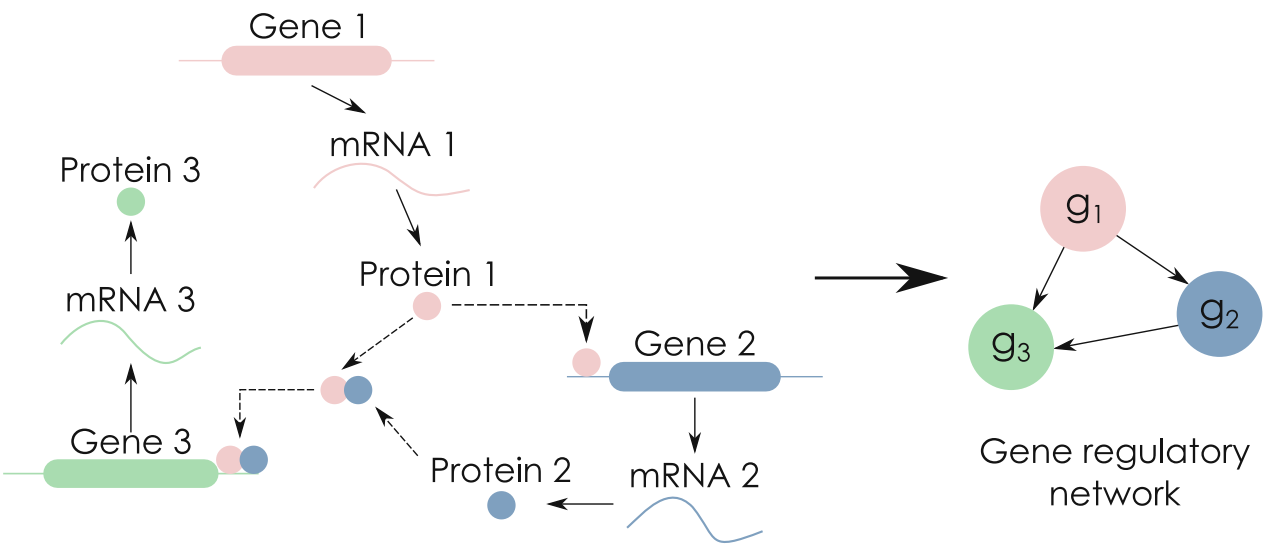
\includegraphics[scale = 0.4]{Figures/Intro/network.PNG}
	    \caption{Illustration schématique d'un réseau de régulation entre 3 gènes \scriptsize \cite{sanguinetti2019gene}}
	    \label{fig:my_label}
	\end{figure}
\end{frame}



\begin{frame}{Exemple de réseau de régulation chez Arabidopsis}

\begin{center}
    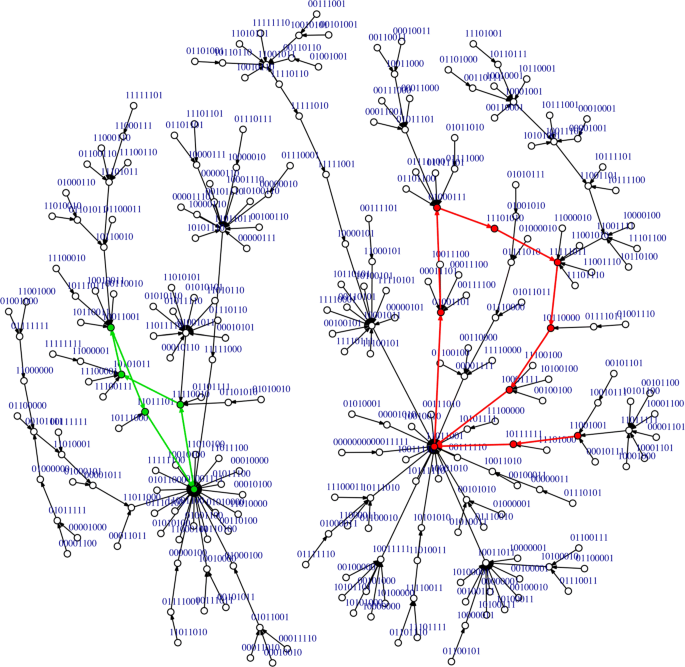
\includegraphics[scale = 0.27]{Figures/Intro/arabidopsis_gene_network.png} 
\end{center}

\vspace{-0.5cm}

\begin{tiny}
Timmermann, T., González, B. \& Ruz, G.A. Reconstruction of a gene regulatory network of the induced systemic resistance defense response in Arabidopsis using boolean networks. BMC Bioinformatics 21, 142 (2020). 
\end{tiny}
%https://doi.org/10.1186/s12859-020-3472-3

\end{frame}

	
	
\begin{frame}{Exemple de réseau de régulation chez Arabidopsis}
\begin{center}
    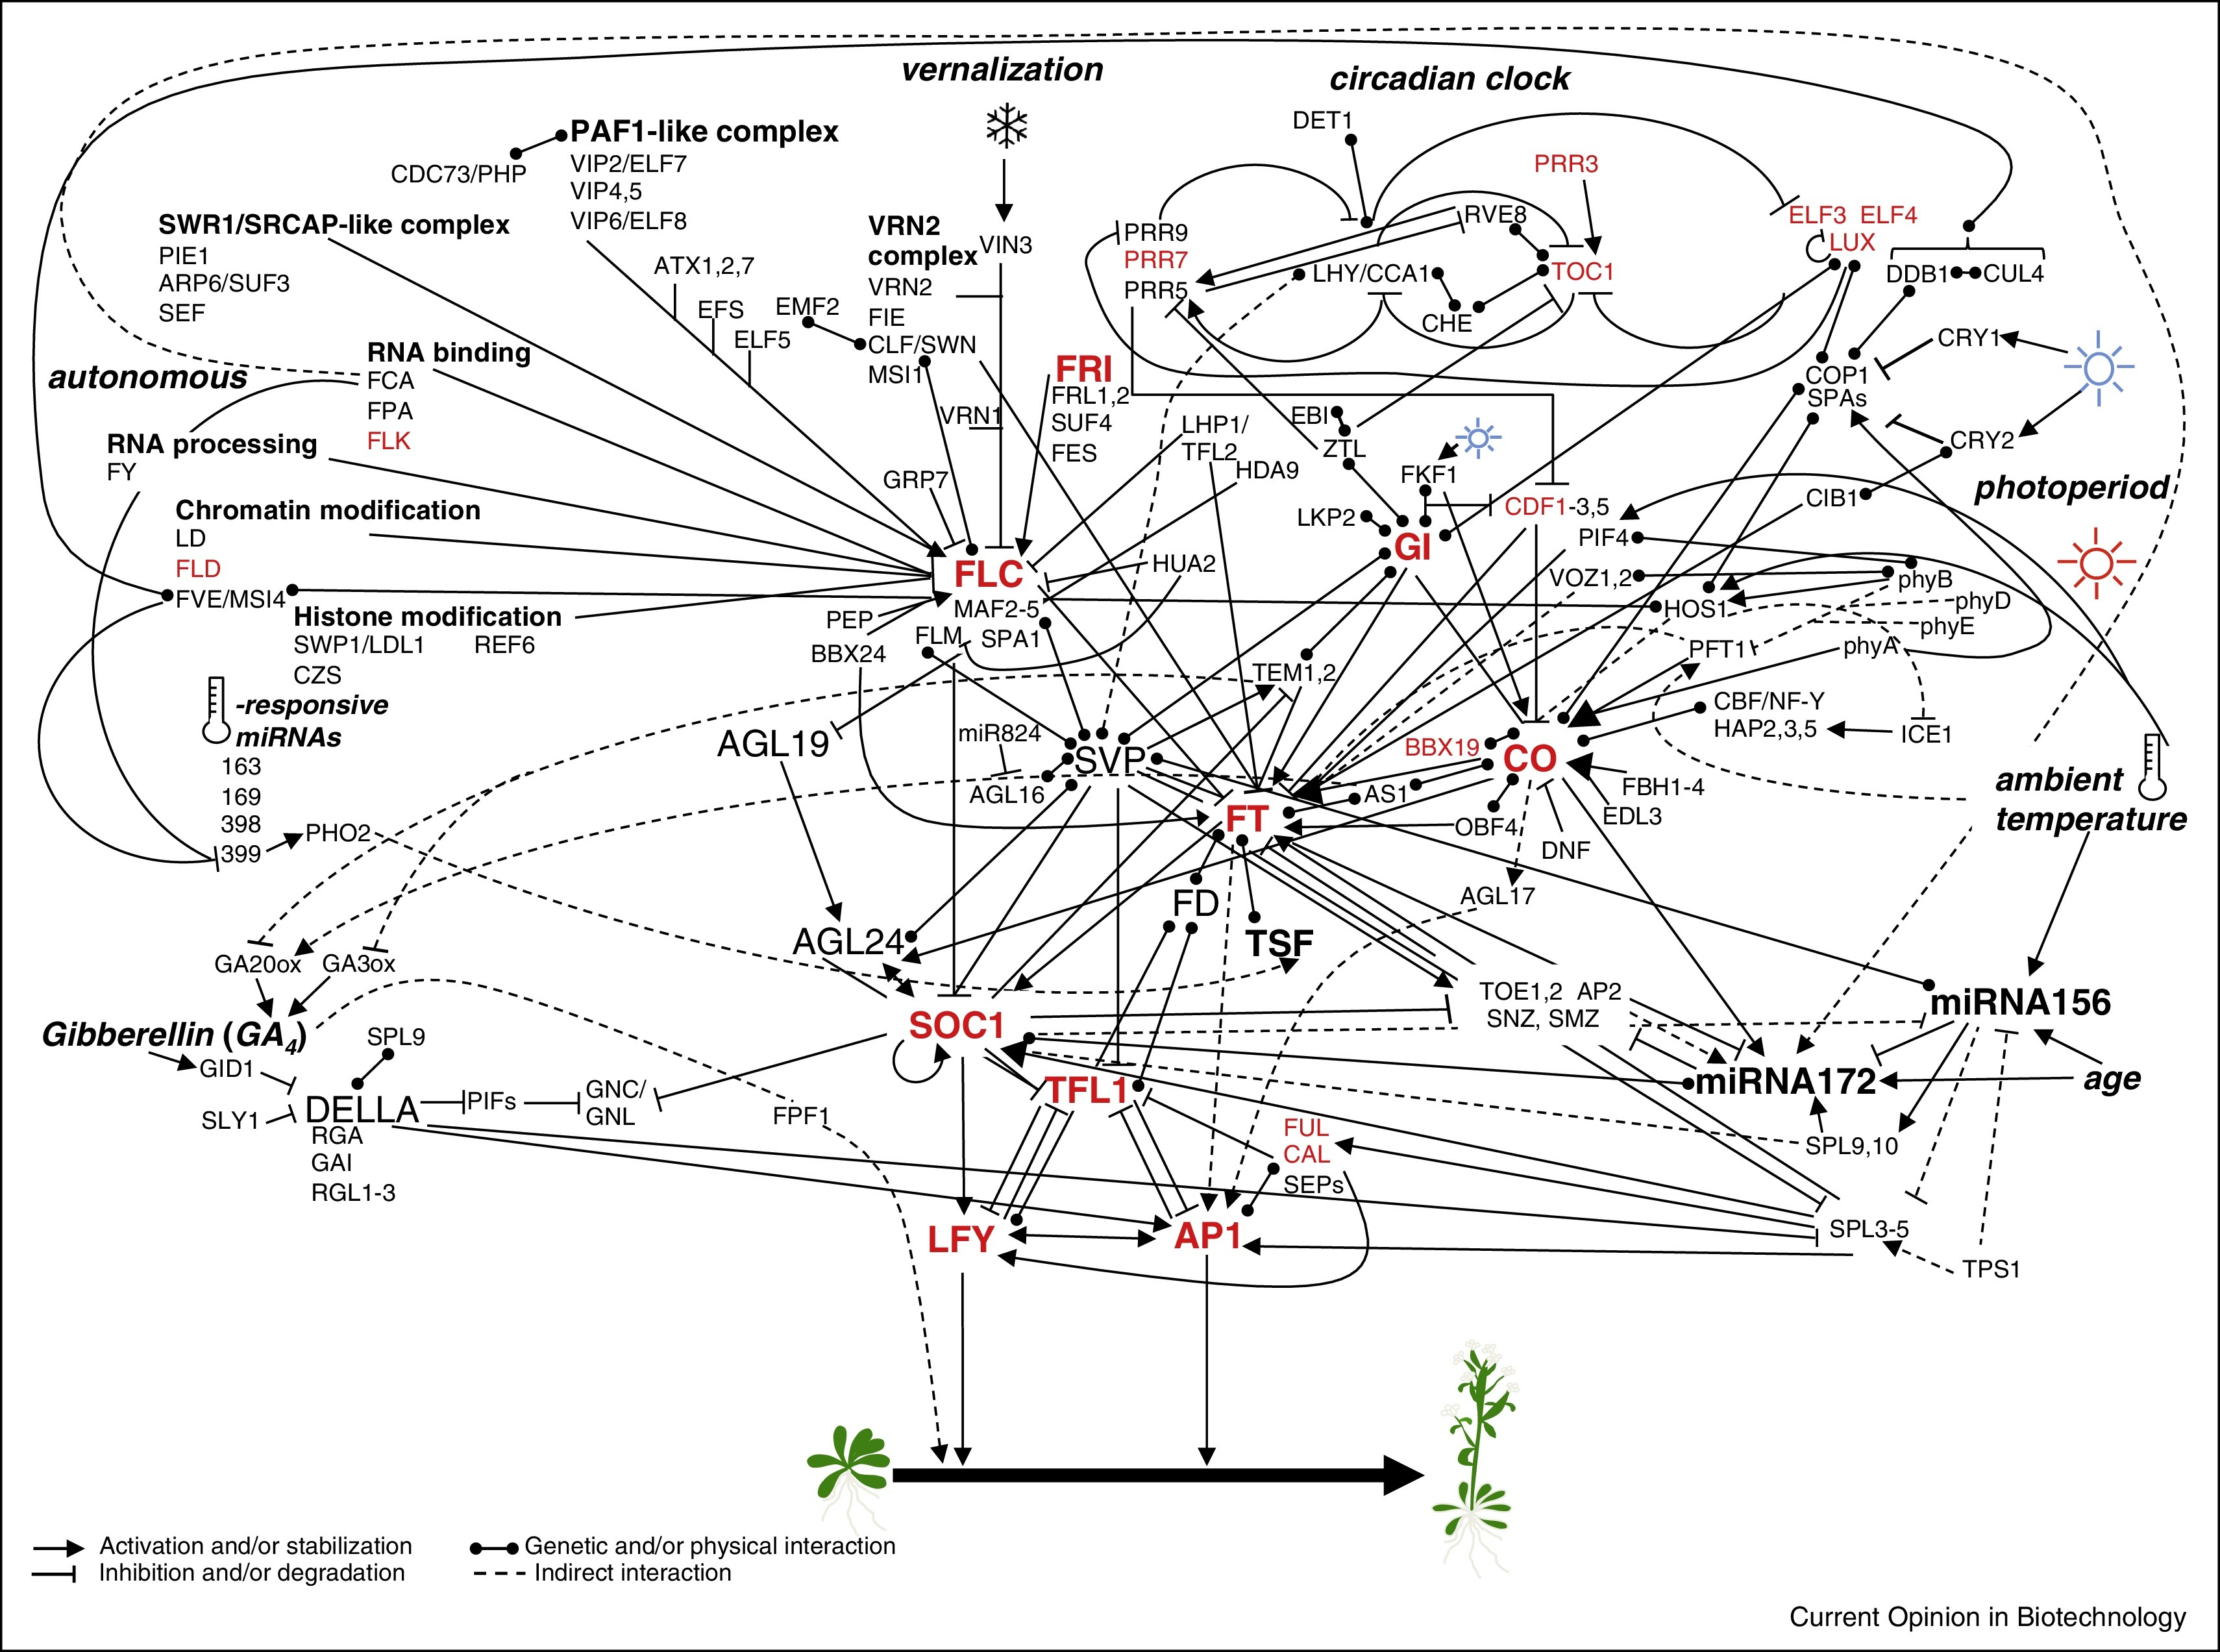
\includegraphics[scale = 0.45]{Figures/Intro/flowering-network-in-arabidopsis.jpeg}
 \end{center}
 
\begin{tiny}
    Flowering time gene network with known genetic and epigenetic regulators in Arabidopsis thaliana.\\
    Blümel, et al., 2015, Current Opinion in Biotechnology
    \end{tiny}
\end{frame}

	
	
\begin{frame}
\frametitle{Utilisation des réseaux en génomique fonctionnelle}
\vspace{-0.1cm}
\hspace{6.3cm}	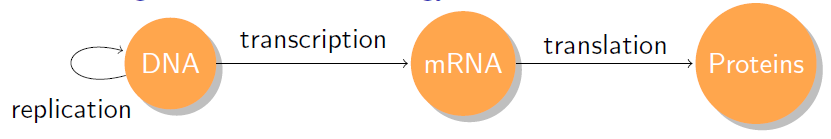
\includegraphics[width=5cm]{Figures/Intro/DogmeBM.png} 
\vspace{-0.5cm}		
\begin{itemize}
\item Différents domaines d'application
\begin{itemize}
\item \textcolor{Periwinkle}{Biologie fondamentale}
\begin{itemize}
\item Fonction et interaction des gènes et proteines (annotations, base de données), Machinerie cellulaire
\end{itemize}
\item \textcolor{Periwinkle}{Santé, Médecine}
\begin{itemize}
\item Diagnostique (ex: type de tumeur cancéreuse), Pronostique (ex: analyse de survie), Thérapie (ex: prédiction de la réponse à un traitement, médecine personnlisée)
\end{itemize}
\item \textcolor{Periwinkle}{Biologie végétale} 
\begin{itemize}
\item Agriculture, alimentation
\end{itemize}
\end{itemize}

\item Différents niveaux d'observation
\begin{itemize}\small
\item \textcolor{Periwinkle}{Génome} : analyse de séquence (ex: détection de motifs)
\item \textcolor{Periwinkle}{Transcriptome} : quantité d'ARN messager
\item \textcolor{Periwinkle}{Protéome} : quantité de protéines / interactions et fonctions des protéines
\end{itemize}
	
\end{itemize}
\end{frame}


	\begin{frame}{Données pour l'inférence d'un GRN}
\begin{itemize}
   \item Les \textbf{données de séquences génomiques} ... (PWM, JASPAR, ...)
    \pause
    \item Les \textbf{données de fixation} des régulateurs sur les promoteurs cibles sont très utiles, cependant : 
    
    \begin{itemize}\scriptsize
        \item Leur génération est relativement chère, contraignante donc faisable sur un \textbf{nombre très restreint de régulateurs}. 
        \item La fixation d'un TF n'implique pas régulation, et la régulation n'implique pas la fixation. (Interactions distantes, transcientes, coopération...)
    \end{itemize}
      \pause
    
    \item Les \textbf{données d'expression} :
    
    \begin{itemize}\scriptsize
        \item Leur mesure tous les gènes d'un organisme est plus accessible, via puces ou RNA-Seq.
        \item L'expression est une conséquence indirecte, il faut donc "démêler", "deviner", ce qui est de la régulation, ou ce qui est de la co-expression fortuite ou induite par des régulations communes
        \end{itemize}
\end{itemize}
	\end{frame}
	
	
	

\begin{frame}{Données pour l'inférence d'un GRN}
    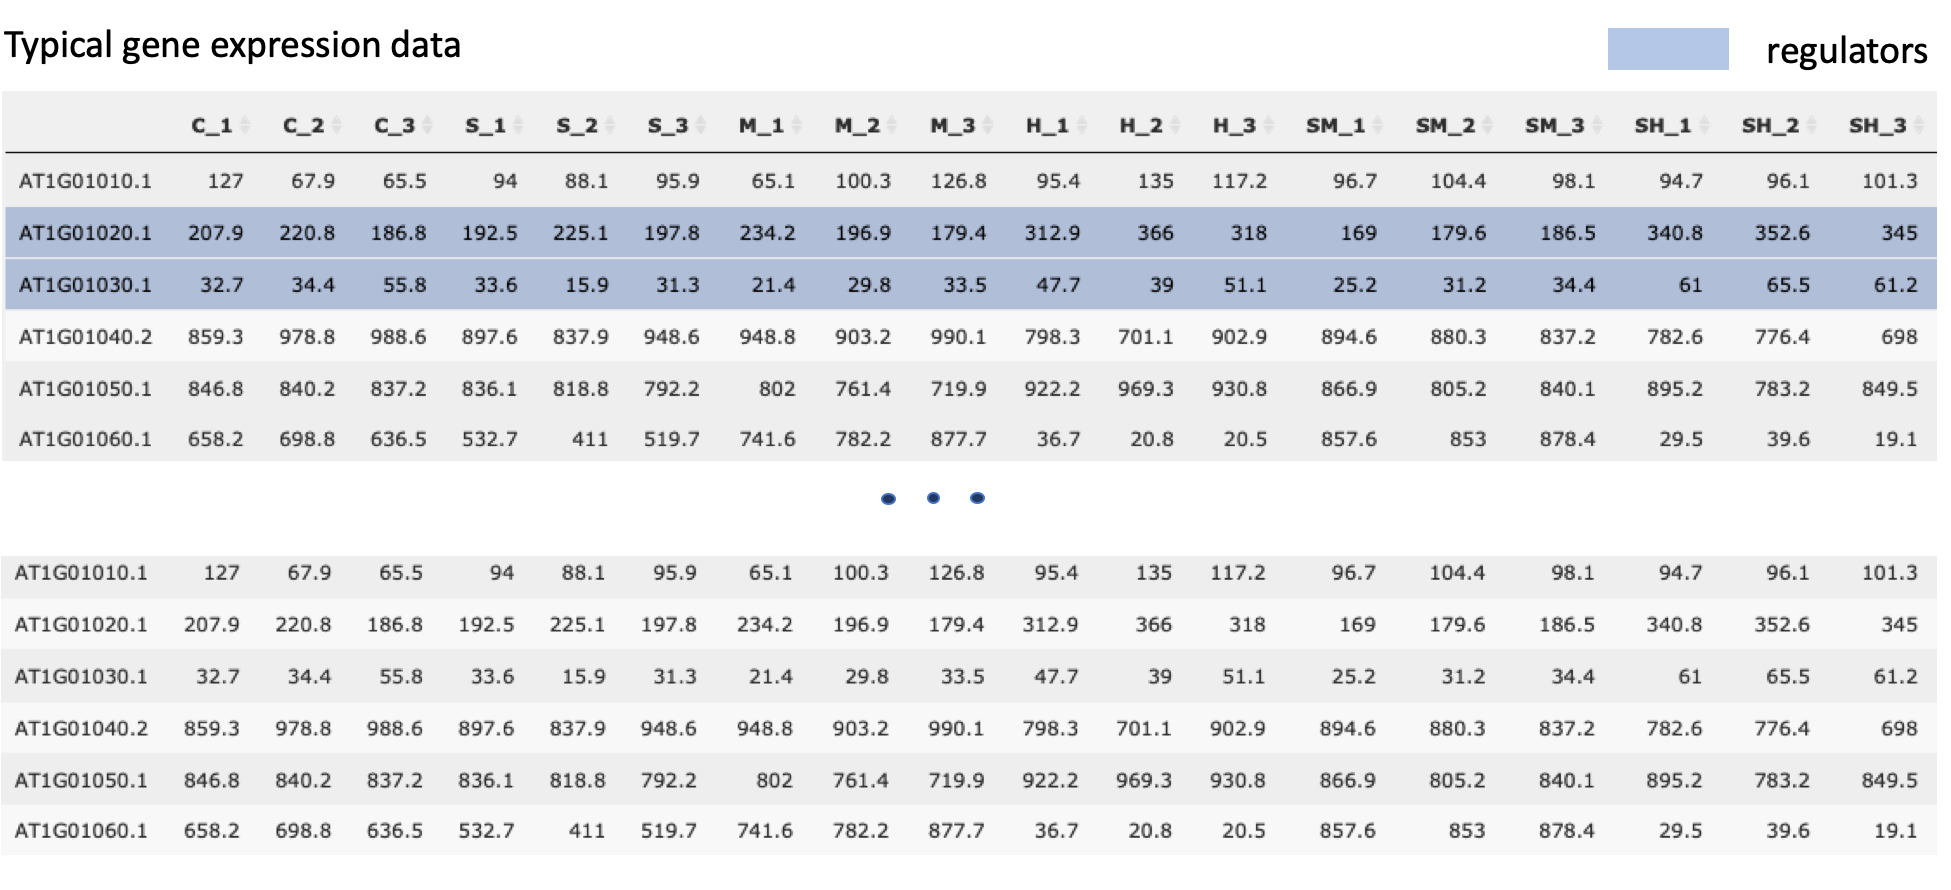
\includegraphics[scale = 0.17]{Figures/Intro/expression_data.png}
\end{frame}

	
\subsection{Réseau de co-expression vs réseau de régulation}



\begin{frame}
\frametitle{Modélisation et inférence ? }
\vspace{-0.1cm}
\begin{center}
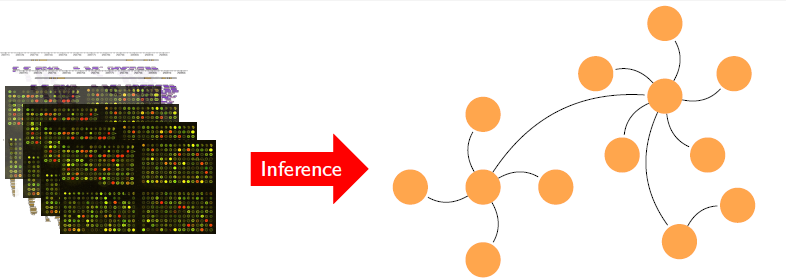
\includegraphics[width=9cm]{Figures/Intro/inference.png}
\end{center}
\vspace{-0.15cm}
\begin{itemize}\small
\item Que représentent les noeuds ? les arêtes ?
\item Biologiquement ? Statistiquement ? 
\item Est-ce que les arêtes sont orientées ? (causalité)
\item Le réseau est-il statique ? dynamique ? 
\item Comment les données ont-elles été générées ? (temporelles (time course), différentes conditions expérimentales (steady state), réplicats)
\end{itemize}

\end{frame}

\begin{frame}
\frametitle{Modélisation et inférence ? }
\vspace{-0.1cm}
\begin{center}
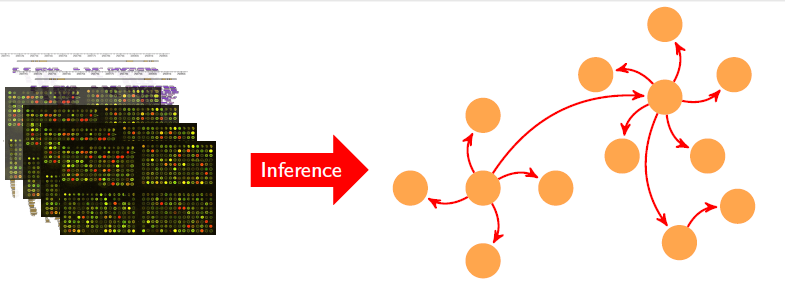
\includegraphics[width=9cm]{Figures/Intro/inference_oriente.png}
\end{center}
\vspace{-0.15cm}
\begin{itemize}\small
\item Que représentent les noeuds ? les arêtes ?
\item Biologiquement ? Statistiquement ? 
\item Est-ce que les arêtes sont orientées ? (causalité)
\item Le réseau est-il statique ? dynamique ? 
\item Comment les données ont-elles été générées ? (temporelles (time course), différentes conditions expérimentales (steady state), réplicats)
\end{itemize}

\end{frame}

\begin{frame}{Le problème de la grande dimension (p $>$ n) }


\small \textbf{Si les données d'expression à disposition contiennent $p$ gènes et $n$ conditions expérimentales:}

\begin{itemize} \small 
    \item les données à disposition sont de l'ordre de $n*p$
    \item les données que nous aimerions obtenir, c.a.d les liens entre les gènes, sont de l'ordre de  $p*p$
\end{itemize}

Si $p>n$, le volume d'information que nous essayons de reconstruire est plus grand que le volume d'information que nous avons à disposition! Et c'est très souvent le cas.

\center
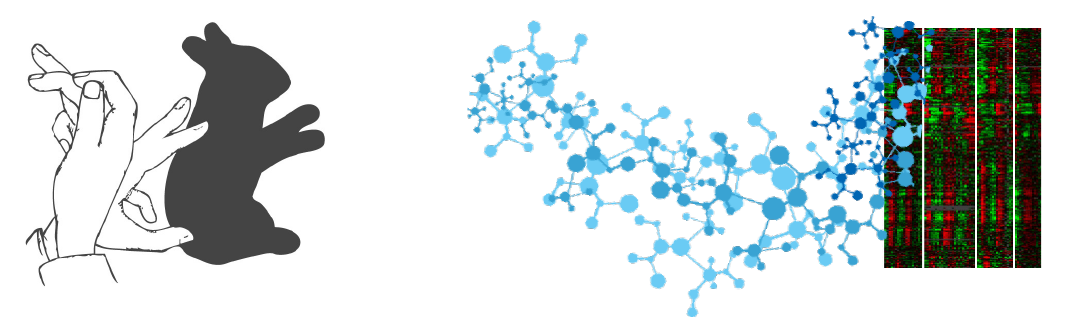
\includegraphics[scale = 0.2]{Figures/Intro/shadowplay.png}
    
\end{frame}

\begin{frame}{Régulation $\neq$ Co-expression}
	\begin{columns}[T] % align columns
        \begin{column}{.45\textwidth}
            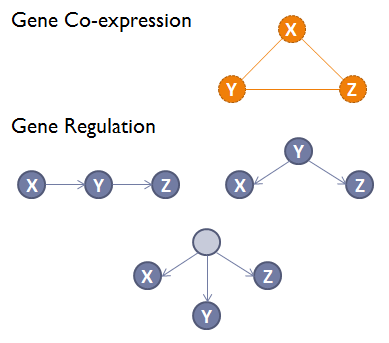
\includegraphics[scale = 0.65]{Figures/Intro/Gene_co-expression_vs_regulation.png}
        \end{column}
        \hfill%
        \begin{column}{.45\textwidth}
            \textcolor{orange}{\textbf{Réseau de co-expression:}}
                    \begin{itemize}
                      \item Arêtes non orientées
                      \item Arêtes reliant tous les types de gènes
                    \end{itemize}
            \vspace{0.5cm}
            \textcolor{Periwinkle}{\textbf{Réseau de régulation:}}
            \begin{itemize}
                  \item Arêtes orientées
                  \item Arêtes partant des gènes régulateurs vers les gènes cibles
            \end{itemize}
        \end{column}%
\end{columns}
\end{frame}
	
	
\begin{frame}{Signification d'un réseau de régulation}
\begin{itemize}
    \item Les réseaux de régulation sont \textbf{plus contraints} que les réseaux de co-expression, et portent une signification biologique \textbf{plus précise}
    \item Les réseaux de régulation recherchent plus de \textbf{causalité} dans l'explication des dépendances transcriptionnelles
    \onslide<2> 
    \vspace{0.5cm}
    \begin{alertblock}{Attention aux interprétations}
    La causalité reste toute fois difficile à atteindre
    \end{alertblock}
    
    
\end{itemize}
	\end{frame}


	



    
\section{Réseaux de co-expression}


    	%\include{regression_files/co-expression-methods}
    	

    	
\section{Inférence de GRN par régression}


    \subsection{La régression}


	\begin{frame}
   \frametitle{Utiliser un \textbf{\textit{a priori} biologique}}
    	\vspace{-0.4cm}
    	\begin{center}
    	    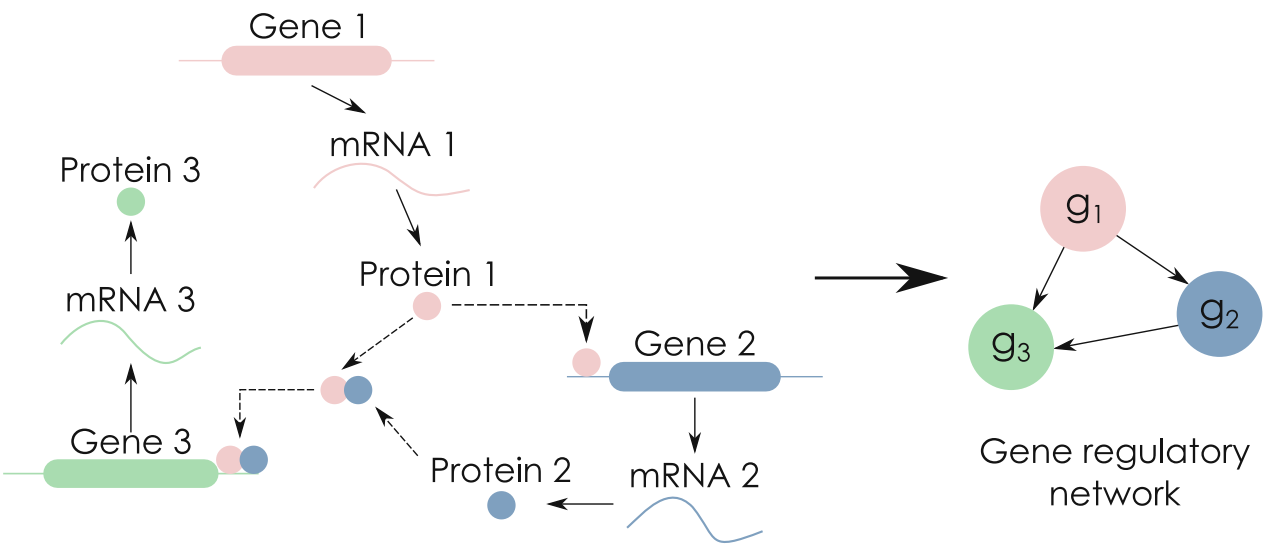
\includegraphics[scale = 0.33]{Figures/Intro/network.PNG}
    	\end{center}
    	\scriptsize \cite{sanguinetti2019gene}
    	
    	\onslide<2> 
    	
    	\begin{center}
\small    	
    	On considère que les niveaux d'expression des régulateurs $g_{1}, g_{2}$ vont permettre de prédire et d'expliquer les niveaux d'expression de $g_{3}$
    	\end{center}
	\end{frame}
	
	
	\begin{frame}{Qu'est-ce qu'une régression?}
	La régression est une procédure statistique visant à établir la relation entre
	
		\begin{enumerate}
		    \item Une \textbf{variable d'intérêt}, également désignée comme variable réponse ou variable dépendante
		    
		    \item Une ou plusieurs \textbf{variables prédictives}, également désignées comme covariables, prédicteurs, ou variables indépendantes
		\end{enumerate}
	\end{frame}
	
	
	\begin{frame}{Qu'est-ce qu'une régression?}
	La régression est une procédure statistique visant à établir la relation entre
	
		\begin{enumerate}
		    \item Une \textbf{variable d'intérêt} $Y$ : vecteur d'observations de la réponse
		    
		    \item Une ou plusieurs \textbf{variables prédictives} $X$ :  vecteur ou matrice de prédicteurs pour chaque observation
		\end{enumerate}
		Le lien entre $X$ et $Y$ se fait au moyen d'une fonction $f$, estimée lors de la procédure de régression, telle que:
		\Large
		\begin{equation*}
		    Y_i = \textcolor{orange}{\textbf{f}}(X_i) + \epsilon_i
		\end{equation*}
		\small
		Avec $i$ allant de 1 à $N$, et $\epsilon_i$ l'erreur (ou résidus) du modèle, soit la variation de $Y$ non expliquée par les prédicteurs $X$.

	\end{frame}
	
	
	\begin{frame}{Exemple de régression : la biomasse}
	La régression est une procédure statistique visant à établir la relation entre
	
	
		\begin{enumerate}
		    \item Une \textbf{variable d'intérêt} $Y$ : la \textbf{biomasse} d'Arabidopsis thaliana 
		    
		    \centering 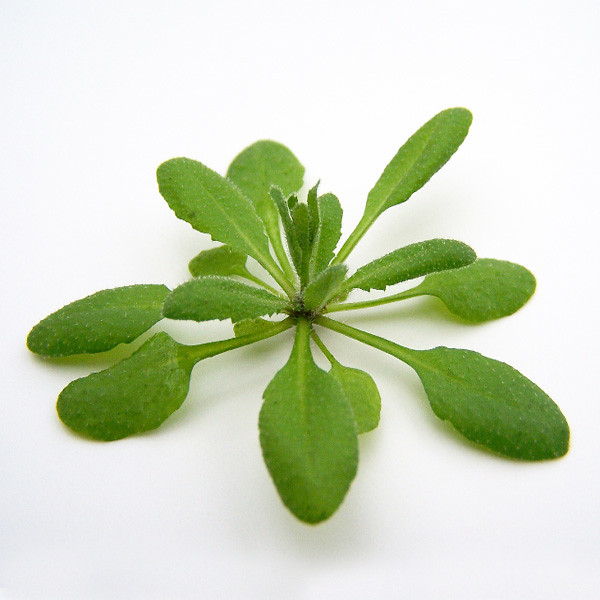
\includegraphics[scale = 0.041]{Figures/Intro/Arabidopsis.jpg}
		
		    
		    \item Une ou plusieurs \textbf{variables prédictives} $X$ :  \textbf{L'apport en nitrate, la température, l'humidité}, etc.
		\end{enumerate}
		
		
		\Large
		
		\begin{equation*}
		    Biomasse_i = \textcolor{orange}{\textbf{f}}(Nitrate_i) + \epsilon_i
		\end{equation*}
		
		\small
		Avec $i$ allant de 1 à $N$ correspondant à chacune des plantes du jeu de données, et $\epsilon_i$ la variation de biomasse non expliquée par l'apport en nitrate, la température, l'humidité, etc.

	\end{frame}
	
	
	\begin{frame}{Représentation graphique}
	Cas d'une régression \textbf{linéaire} à un prédicteur : $Y_i = \textcolor{orange}{\textbf{a}} + \textcolor{orange}{\textbf{b}}X_i + \epsilon_i$
	
	\vspace{0.5cm}
	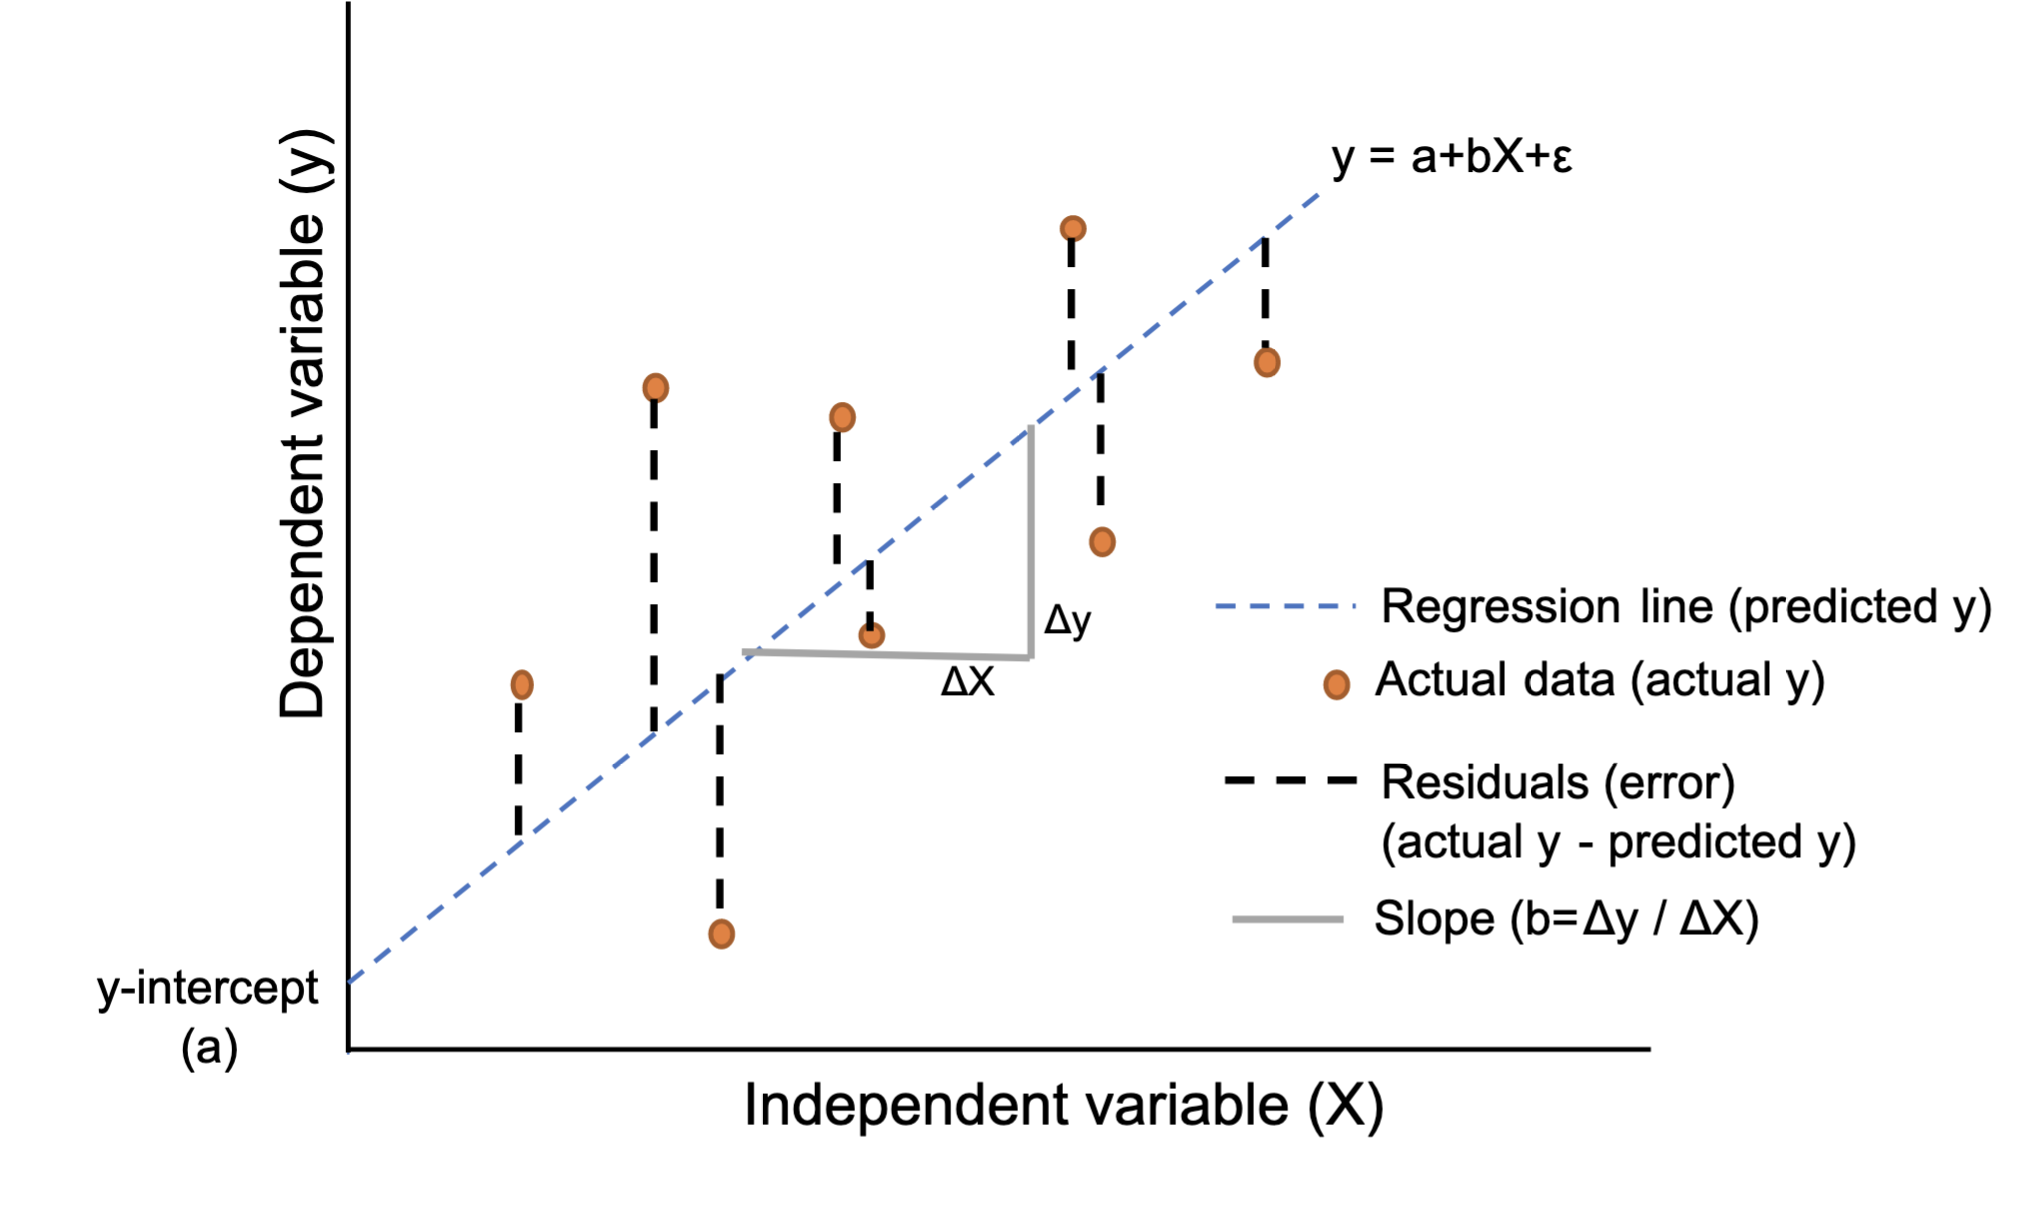
\includegraphics[scale=0.275]{Figures/Intro/regressionLine.png}
	\end{frame}
	
	
	\begin{frame}{Régression simple et régression multiple}
    	Cas d'une régression \textbf{linéaire} à deux prédicteurs (sans interaction): 
    	\begin{equation*}
    	    Biomasse_i = \textcolor{orange}{\textbf{a}} + \textcolor{orange}{\textbf{b}}Nitrate_i +\textcolor{orange}{\textbf{c}}Temperature_i + \epsilon_i
    	\end{equation*}
    	
    	\vspace{1cm}
    	\onslide<2> 
    	
    	Cas d'une régression \textbf{linéaire} à deux prédicteurs (avec interaction): 
    	\begin{equation*}
    	    Biomasse_i = \textcolor{orange}{\textbf{a}} + \textcolor{orange}{\textbf{b}}Nitrate_i +\textcolor{orange}{\textbf{c}}Temperature_i + \textcolor{orange}{\textbf{d}}Temperature_i*Nitrate_i + \epsilon_i
    	\end{equation*}
    	
    	
    	
	\end{frame}
	
	\begin{frame}{Remarques}

    	\textbf{Avantages de la régression : }
    	
    	
    	\begin{itemize} \scriptsize
    	\item Possibilité de prédire la variable d'intérêt pour un nouveau set de variables à l'outcome inconnu
    	    \item Quantification du pouvoir prédicteur de chaque variable d'entrée (ex: valeur du coefficient, et test sur la significativité de ce coefficient.)
    	\end{itemize}
    	
    	\onslide<2>
    	
    	
    	\vspace{0.5cm}
    	
    	\textbf{Extensions de la régression linéaire utiles à la suite du cours : }
    	
    	
    	
    	\begin{itemize} \scriptsize
    	
    	\item On peut ajouter des termes de pénalisation lors de l'estimation des coefficients afin de faire de la sélection de variables en grande dimension (lasso)
    	
    	\item La fonction $f$ n'est pas nécessairement une combinaison linéaire du type $\textcolor{orange}{\textbf{a}} + \textcolor{orange}{\textbf{b}}X1_i + \textcolor{orange}{\textbf{c}}X2_i$, mais peut prendre la forme des arbres de régression, des fonctions non linéaires plus adaptées à des questions biologiques complexes

    	\end{itemize}
    	
    	
	\end{frame}
	
	
	
\subsection{Application aux réseaux de gènes}

	
	\begin{frame}{Principe de l'application aux réseaux de gènes}
    	\vspace{-0.4cm}
    	\begin{center}
    	    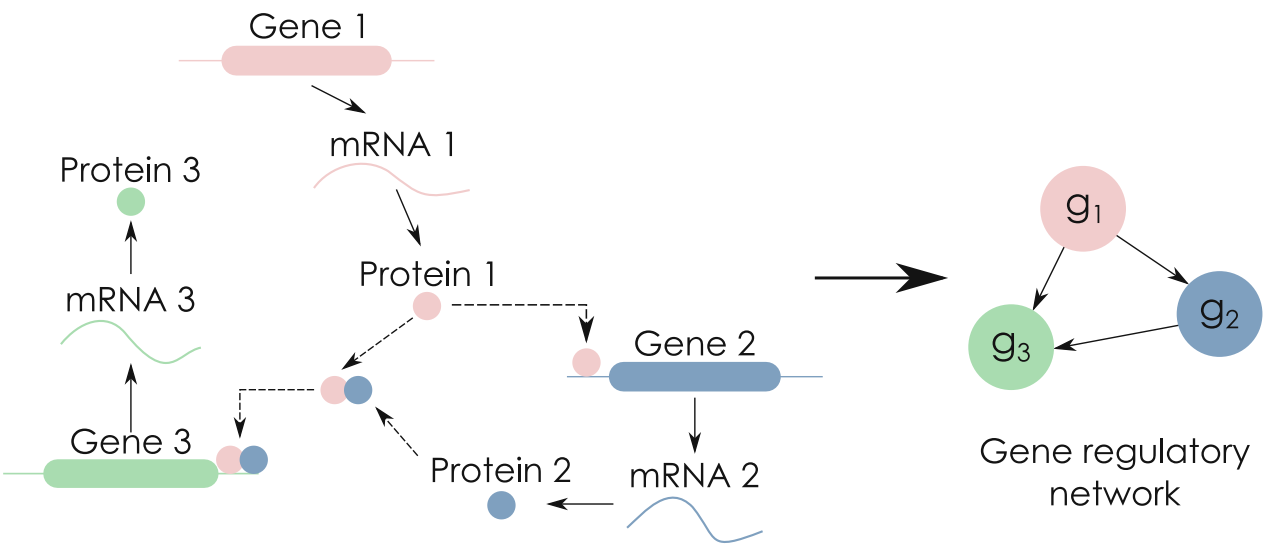
\includegraphics[scale = 0.3]{Figures/Intro/network.PNG}
    	\end{center}
    	
    	\begin{center}
    	\scriptsize 
    	$g_{1i}, g_{2i}$ : niveaux d'expression des régulateurs transcriptionels dans la condition $i$
    	
    	$g_{3i}$  : niveaux d'expression d'un gène cible dans la condition $i$
    	\end{center}
    	\vspace{-0.15cm}
    	\Large
    	\begin{equation*}
    	    g_{3i} = \textcolor{orange}{\textbf{f}}(g_{1i}, g_{2i}) + \epsilon_i
    	\end{equation*}
	\end{frame}
	
	
	\begin{frame}{Principe de l'application aux réseaux de régulation}
    	
    	\begin{center}
    	\scriptsize 
    	$regulators_{i}$ : niveaux d'expression des régulateurs transcriptionels dans la condition $i$
    	
    	$target_{i}$  : niveaux d'expression d'un gène cible dans la condition $i$
    	\end{center}
    	\vspace{-0.15cm}
    	
    	
    	\begin{block}{}
    	\begin{equation*}
    	    target_{i} = \textcolor{orange}{\textbf{f}}(regulators_{i}) + \epsilon_i
    	\end{equation*}
    	\end{block}
    	\vspace{0.25cm}

    	\scriptsize 
    	
    	
    	\textbf{La procédure de construction de réseau est la suivante} : 
    	
    	\begin{enumerate}
    	    \item Pour chaque gène du jeu de données, ajuster à partir des valeurs d'expression la fonction \textcolor{orange}{\textbf{f}}
    	    \item Extraire de \textcolor{orange}{\textbf{f}} les scores (ou valeur d'influence, importance, pouvoir prédictif) des régulateurs sur chaque gène du jeu de données 
    	    \item Sélectionner les scores régulateurs-gènes cibles les plus forts pour construire le réseau final
    	\end{enumerate}
    	
	\end{frame}
	
	
\begin{frame}{Principe de l'application aux réseaux de régulation}
    	
    	\begin{center}
    	\scriptsize 
    	$regulators_{i}$ : niveaux d'expression des régulateurs transcriptionels dans la condition $i$
    	
    	$target_{i}$  : niveaux d'expression d'un gène cible dans la condition $i$
    	\end{center}
    	\vspace{-0.15cm}
    	
    	\begin{block}{}
    	\begin{equation*}
    	    target_{i} = \textcolor{orange}{\textbf{f}}(regulators_{i}) + \epsilon_i
    	\end{equation*}
    	\end{block}
    	\vspace{0.25cm}

    	\scriptsize 
    	Les méthodes basées sur la régression pour inférerer des GRN se différencient par leur choix de modélisation pour $f$.
    	Deux sont présentées dans ce cours : 
    	\vspace{0.25cm}
    	
    	\begin{itemize}
    	    \item \textcolor{orange}{TIGRESS} : Régression linéaire pénalisée avec sélection de stabilité \cite{haury2012tigress}
    	    \item \textcolor{orange}{GENIE3} : Arbres de régression en random forests \cite{genie3}
    	\end{itemize}
\end{frame}
	

	
	
	\section{Exemples de méthodes}

	\subsection{Application aux réseaux de régulation}



\subsection{Exemple de méthodes : TIGRESS et GENIE3}
	
	\begin{frame}{TIGRESS : approche basée sur la régression linéaire}

TIGRESS fait le choix de modélisation suivant : l'expression d'un gène cible peut être modélisée par une c\textbf{ombinaison linéaire} de l'expression des facteurs de transcription :
    \onslide<2->
    
    \begin{equation*}
    	   target_i = \textcolor{orange}{\beta_{target,1}}.TF1_i + \textcolor{orange}{\beta_{target,2}}.TF2_i + ... + \textcolor{orange}{\beta_{target,M}}.TFM_i  + \epsilon_i
    \end{equation*}
    
Avec $TFM_i$ le niveau d'expression du TF numéro M dans la condition $i$.
\vspace{0.3cm}

\onslide<3-> 

\begin{alertblock}{\small Problème : il faut \textbf{refléter la sparsité du problème biologique}}
\small L'expression d'un gène est sensée être expliquée par un nombre limité de TFs, et non tous les TFs du jeu de données $\rightarrow$ \textbf{LARS} (Least-angle regression)
\end{alertblock}

\end{frame}



\begin{frame}{TIGRESS : Modéliser la sparsité}

\begin{alertblock}{\small Problème : il faut \textbf{refléter la sparsité du problème biologique}}
\small L'expression d'un gène est sensée être expliquée par un nombre limité de TFs, et non tous les TFs du jeu de données $\rightarrow$ \textbf{LARS} (Least-angle regression)
\end{alertblock}

\scriptsize
La méthode LARS fonctionne (dans le principe) comme suit :

\begin{enumerate}\small 
    \item Commencer par le modèle nul : $target_i = \alpha + \epsilon_i$
    \item Choisir le $TF_j$ pour lequel la corrélation à $target$ est maximale : $target_i = \alpha + \textcolor{orange}{\beta_{target,j}}.TFj_i + \epsilon_i$
    \item Continuer à ajouter des TFs en choisissant à chaque fois le TF maximisant la prédiction de $target$
    \item S'arrêter lorsque l'on a atteint le nombre de TFs prédicteurs jugé suffisant, ici $L < M$.
\end{enumerate}

\scriptsize
On termine alors avec le modèle suivant, consitué de uniquement L TFs contre M, sans contrainte de spasite : 
 $target_i = \textcolor{orange}{\beta_{target,1}}.TF1_i + \textcolor{orange}{\beta_{target,2}}.TF2_i + ... + \textcolor{orange}{\beta_{target,L}}.TFL_i  + \epsilon_i$


\end{frame}
	
\begin{frame}{TIGRESS : étapes de la procédure}
	\vspace{-0.3cm}
	\begin{overprint}
	 \onslide<1> 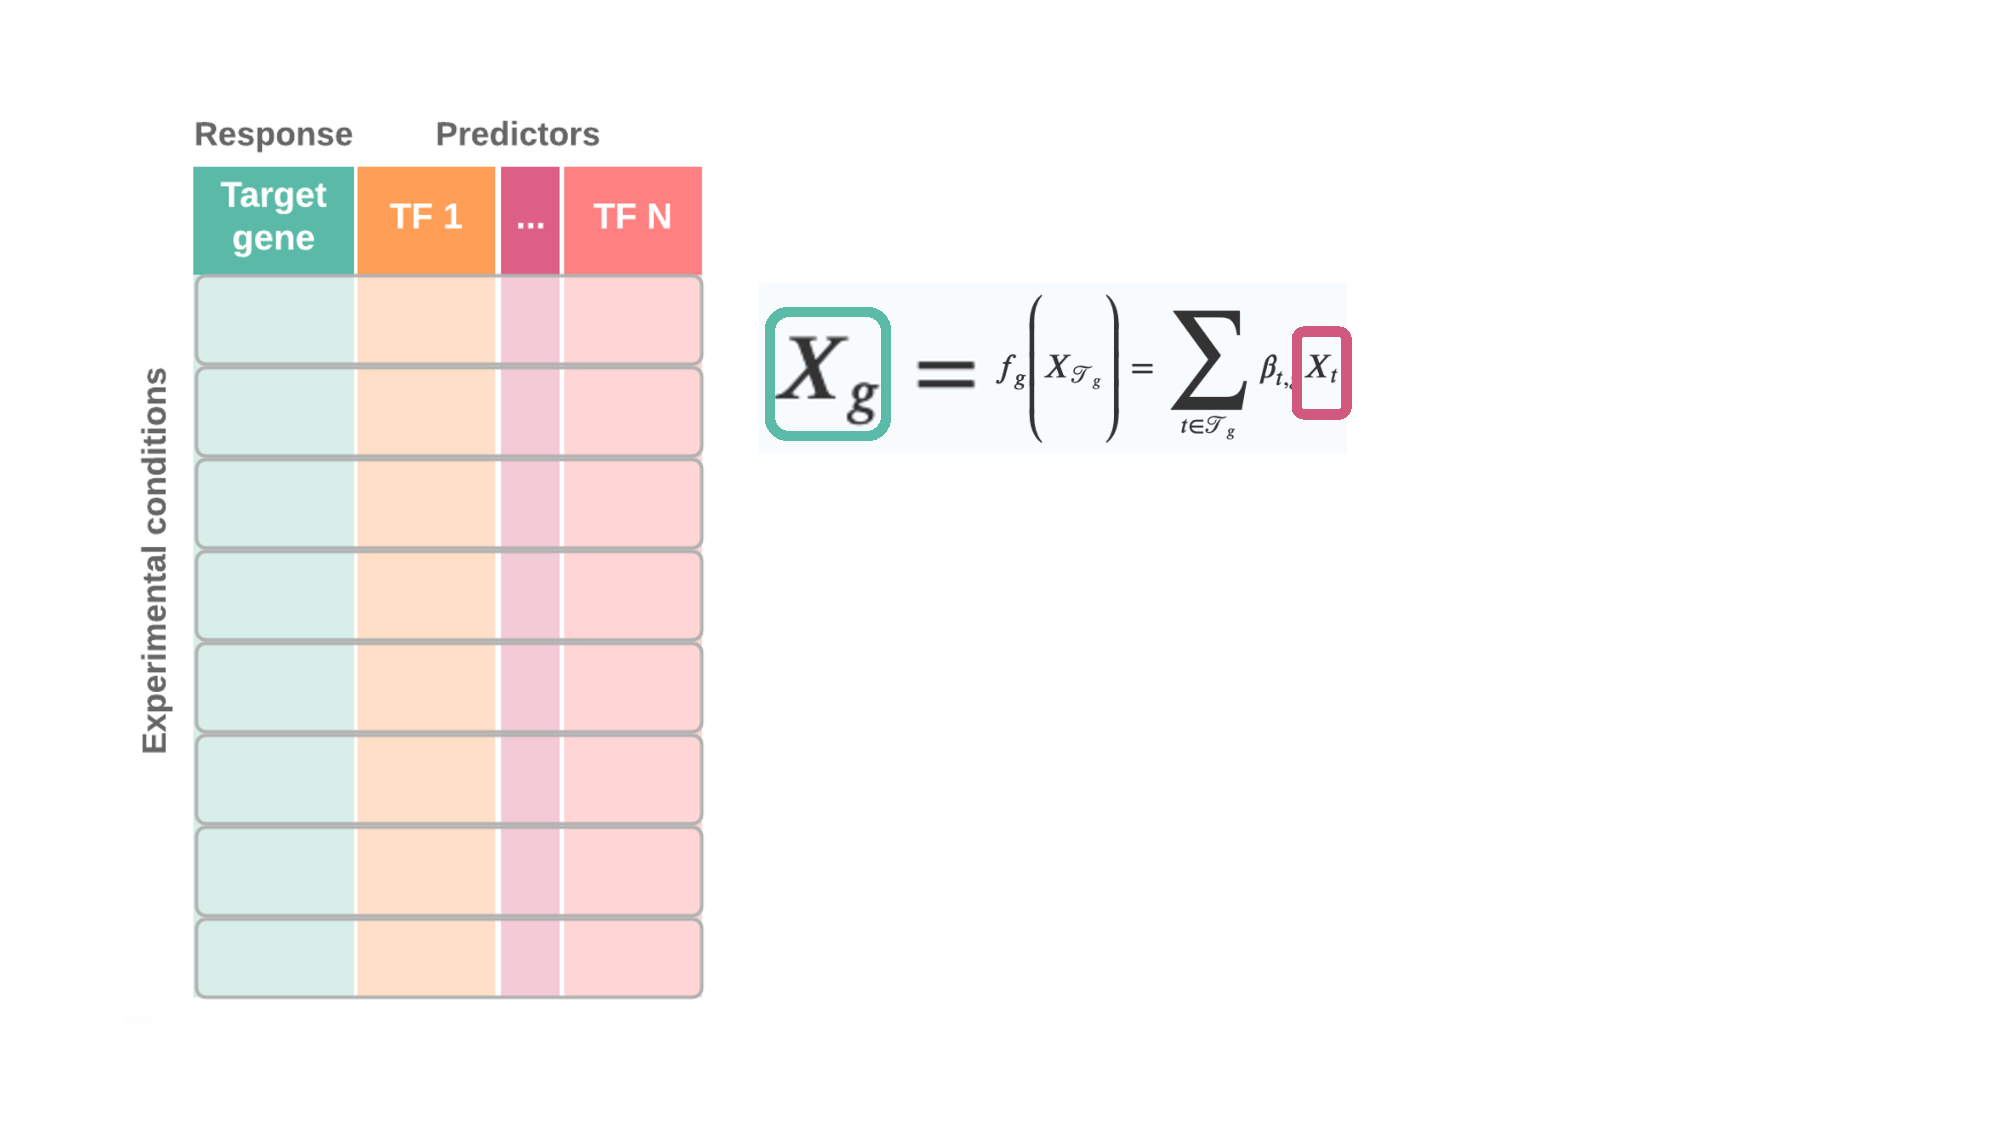
\includegraphics[scale=0.35]{Figures/Regression/tigress_1-1.pdf}
	 \onslide<2> 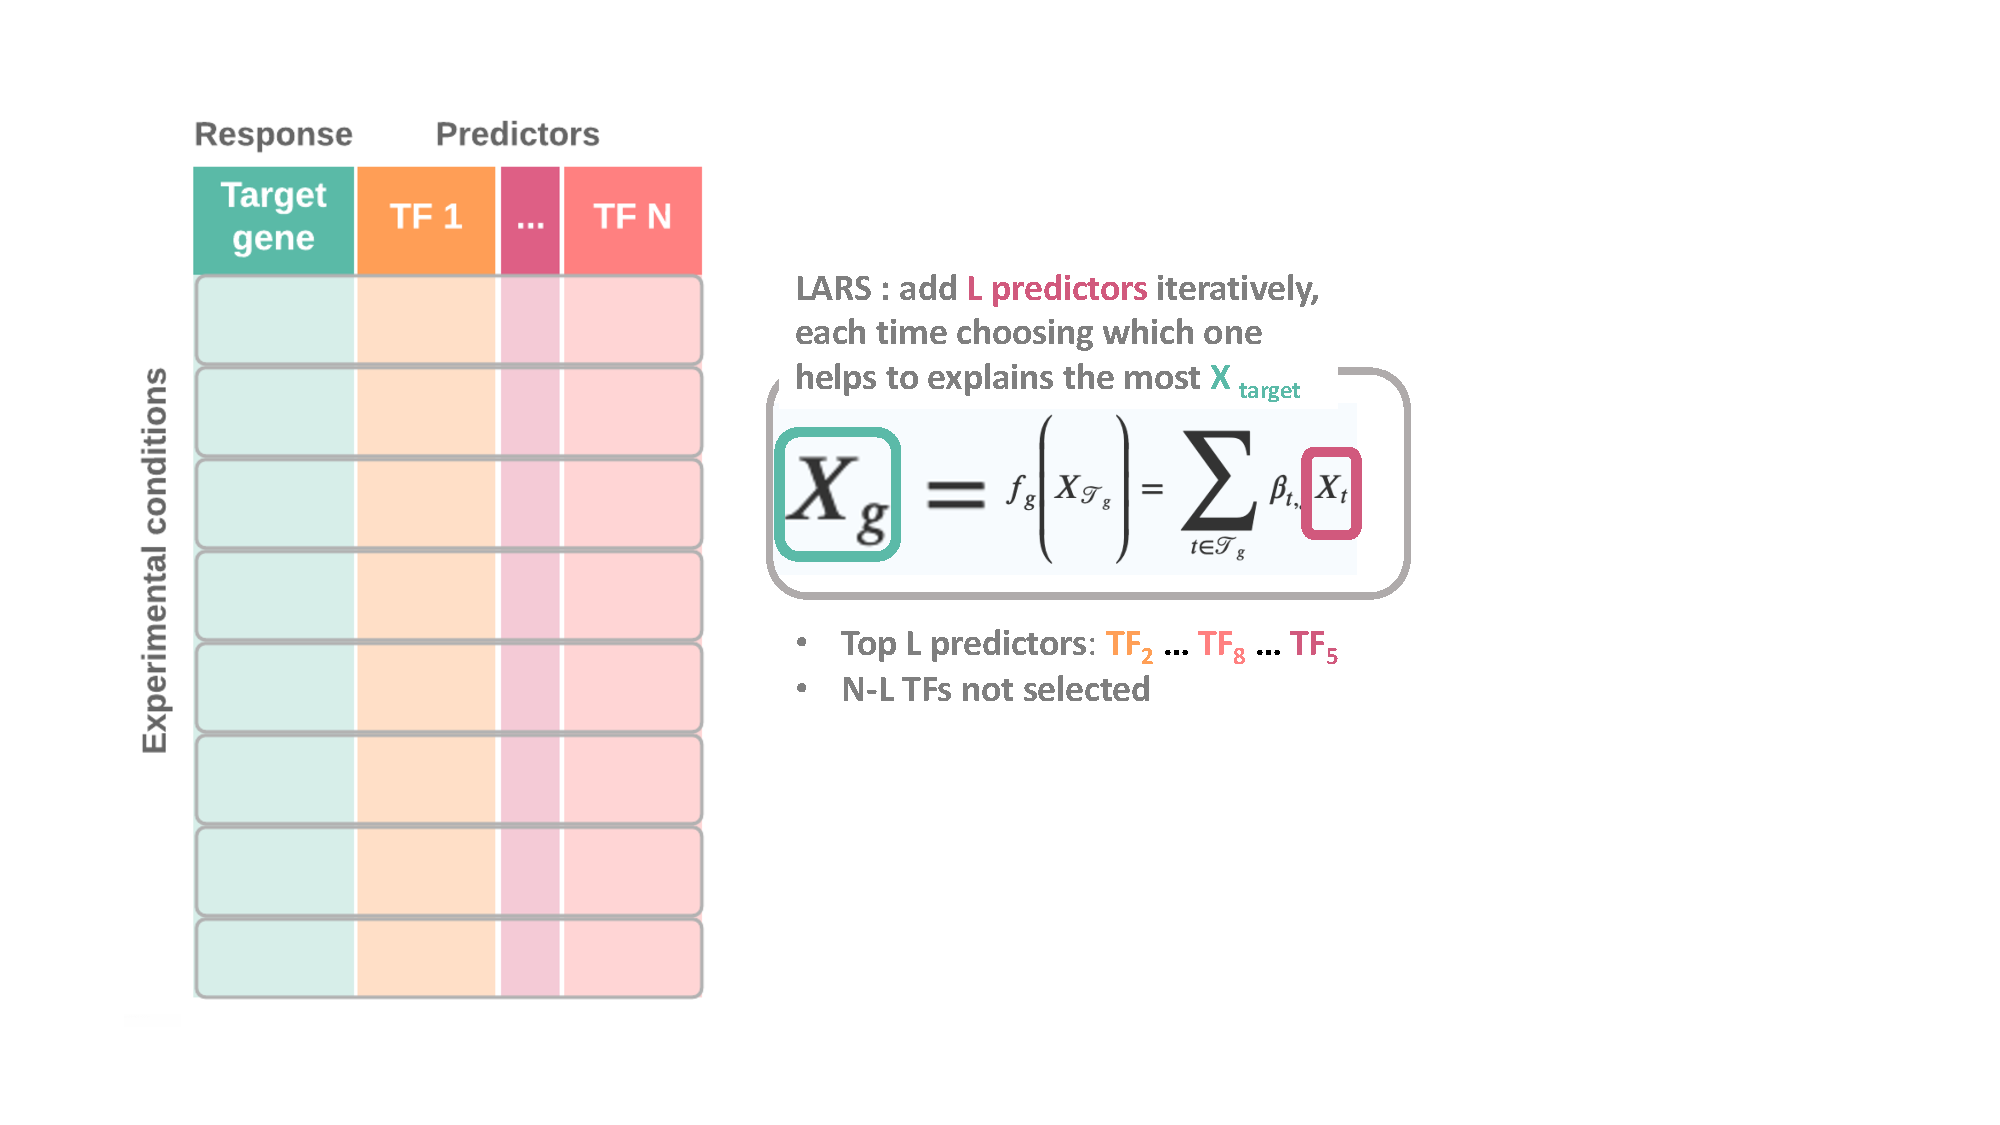
\includegraphics[scale=0.35]{Figures/Regression/tigress_2-2.pdf}
	 \onslide<3> 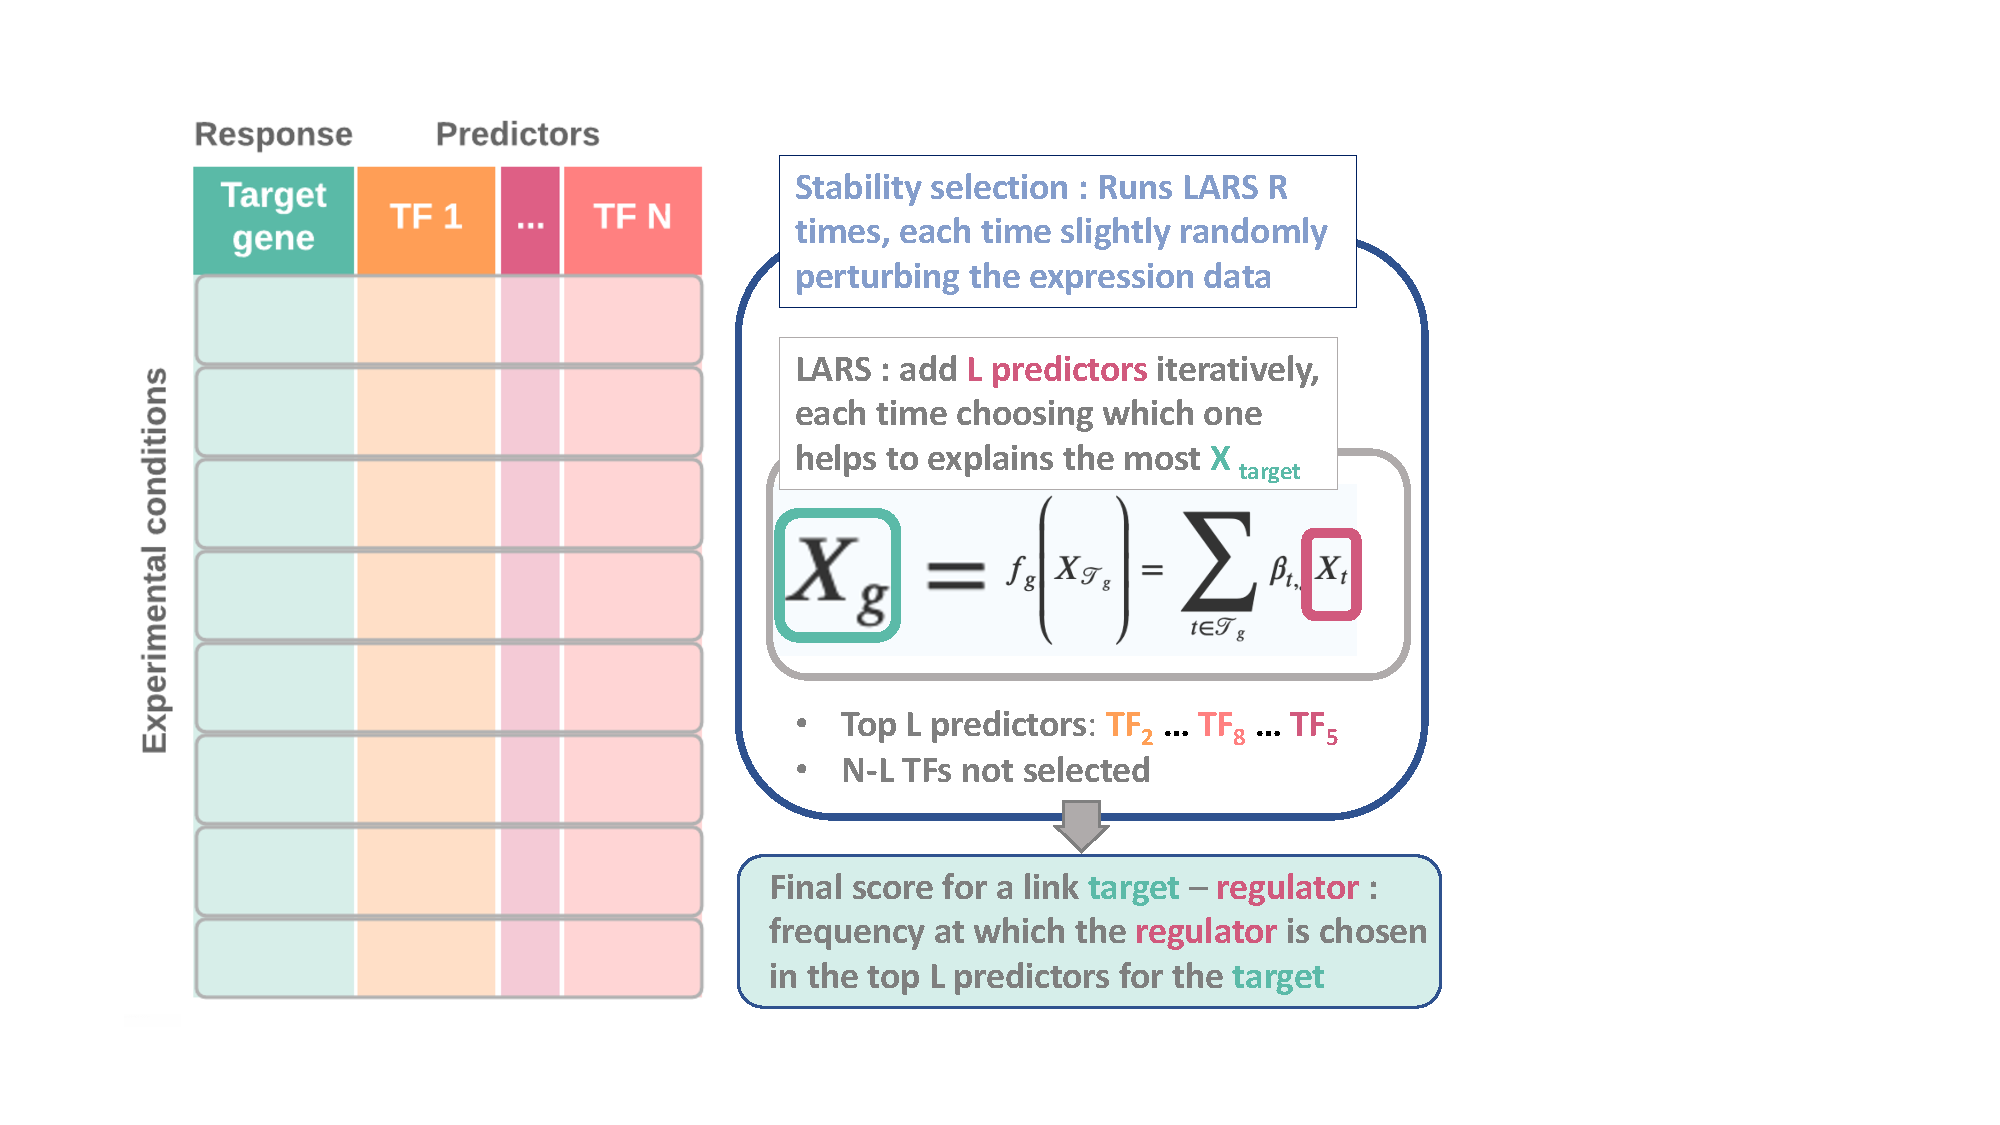
\includegraphics[scale=0.35]{Figures/Regression/tigress_3-3.pdf}
	 \onslide<4> 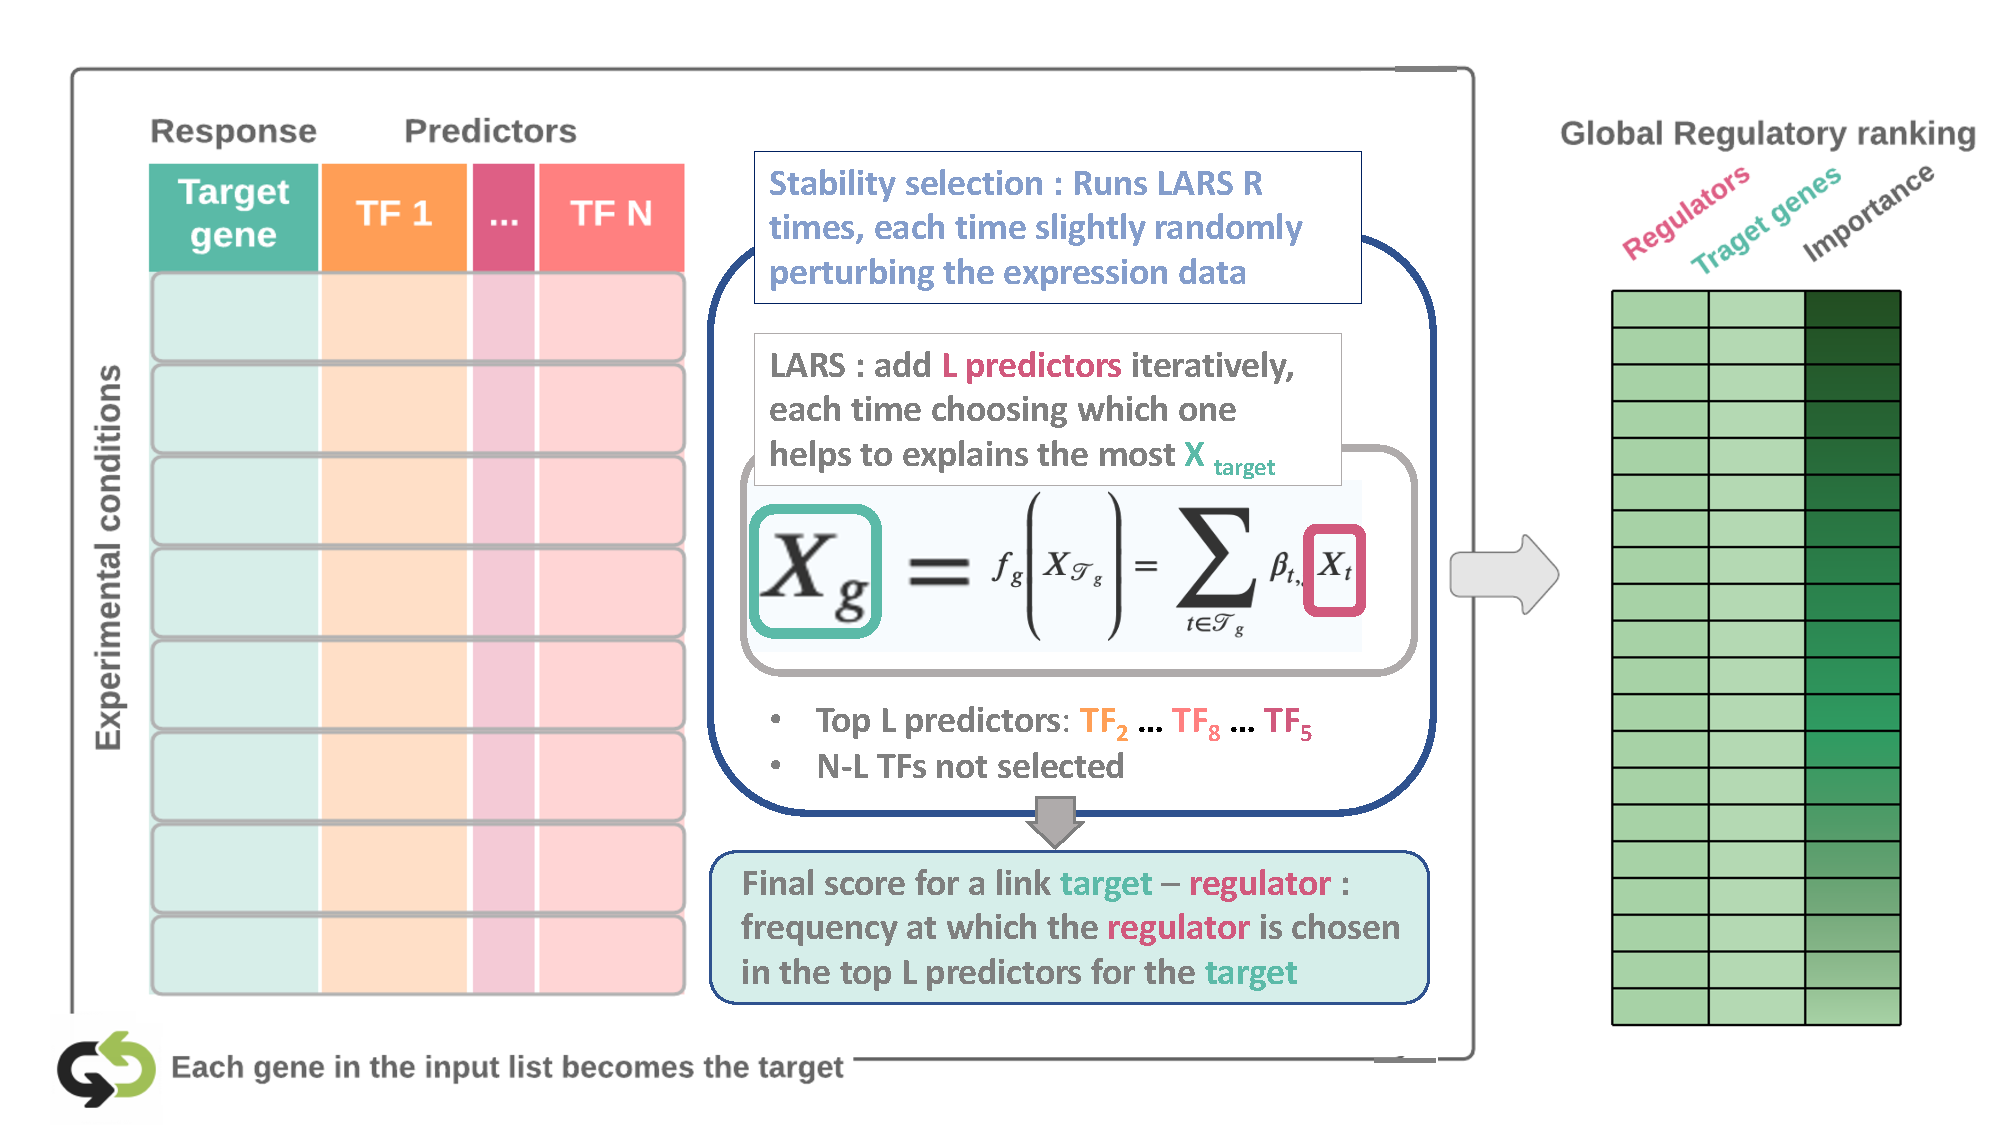
\includegraphics[scale=0.35]{Figures/Regression/tigress_4-end.pdf}
	 
	\end{overprint}
\end{frame}
	
	










\begin{frame}{GENIE3 : approche basée sur les arbres de régression}

GENIE3 fait le choix de modélisation suivant : l'expression d'un gène cible peut être modélisée par une \textbf{combinaison non linéaire} de l'expression des facteurs de transcription :

    \onslide<2->
    
    \begin{equation*}
    	   target_i = \textcolor{orange}{Random Forest}(TF_i) + \epsilon_i
    \end{equation*}
\scriptsize{(On n'a pas de formulation mathématique pour le modèle d'un random forest, qui fonctionne très différemment d'une régression linéaire)}

\small 
Avec $TF_i$ le niveau d'expression de tous les TFs du jeu de données dans la condition $i$.



\begin{block}{\small Avantages par rapport au modèle linéaire}
\begin{itemize}\scriptsize
    \item Peut modéliser des non linéarités dans l'influence de l'expression des régulateurs (ex: le carré de l'expression d'un régulateur, etc)
    \item Peut modéliser des relations de coopération et d'interactions entre TFs
\end{itemize}
\end{block}

\end{frame}



\begin{frame}{GENIE3 : approche basée sur les arbres de régression}


\small Un arbre de régression est construit en choisissant \textbf{des seuils et conditions sur les variables prédictives}.
%Le choix des conditions et seuils sur les variables est fait itérativment, en maximisant la réduction de variabilité de la variable réponse engendrée par l'ajout d'une coniditon.

\begin{columns}
\begin{column}{.45\textwidth}
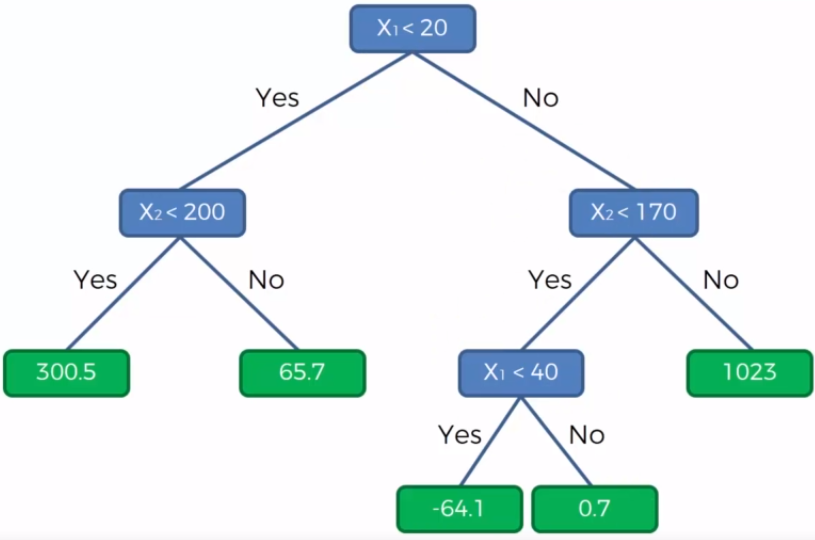
\includegraphics[scale = 0.2]{Figures/Regression/regressionTree.png}
\end{column}
\begin{column}{.45\textwidth}
\small Ajustement d'un arbre de régression
\begin{enumerate}\scriptsize
    \item Choisir la variable et la condition sur cette variable qui permettent de discriminer au mieux les valeurs de la réponse (la variance de la réponse est diminuée)
    \item Réitérer en créant de nouvelles branches, jusqu'à épuisement des variables, ou atteinte de la profondeur d'arbre maximale
\end{enumerate}
\end{column}
\end{columns}
\vspace{0.5cm}

\onslide<2>
\scriptsize \textbf{Random Forest} : un grand nombre d'arbres de régression sont ajustés sur des données échantillonnées légèrement différemment les unes des autres $\rightarrow$ leur consensus permet plus de robustesse dans les prédictions (apprentissage ensembliste)

\end{frame}



\begin{frame}
    \frametitle{GENIE3: étapes de la procédure}
    \small \textbf{Ranking the regulators} according to their \textbf{relevance for predicting} the other genes expression
    \vspace{-0.2cm}
    \begin{center}
        \begin{overprint}
        \onslide<1>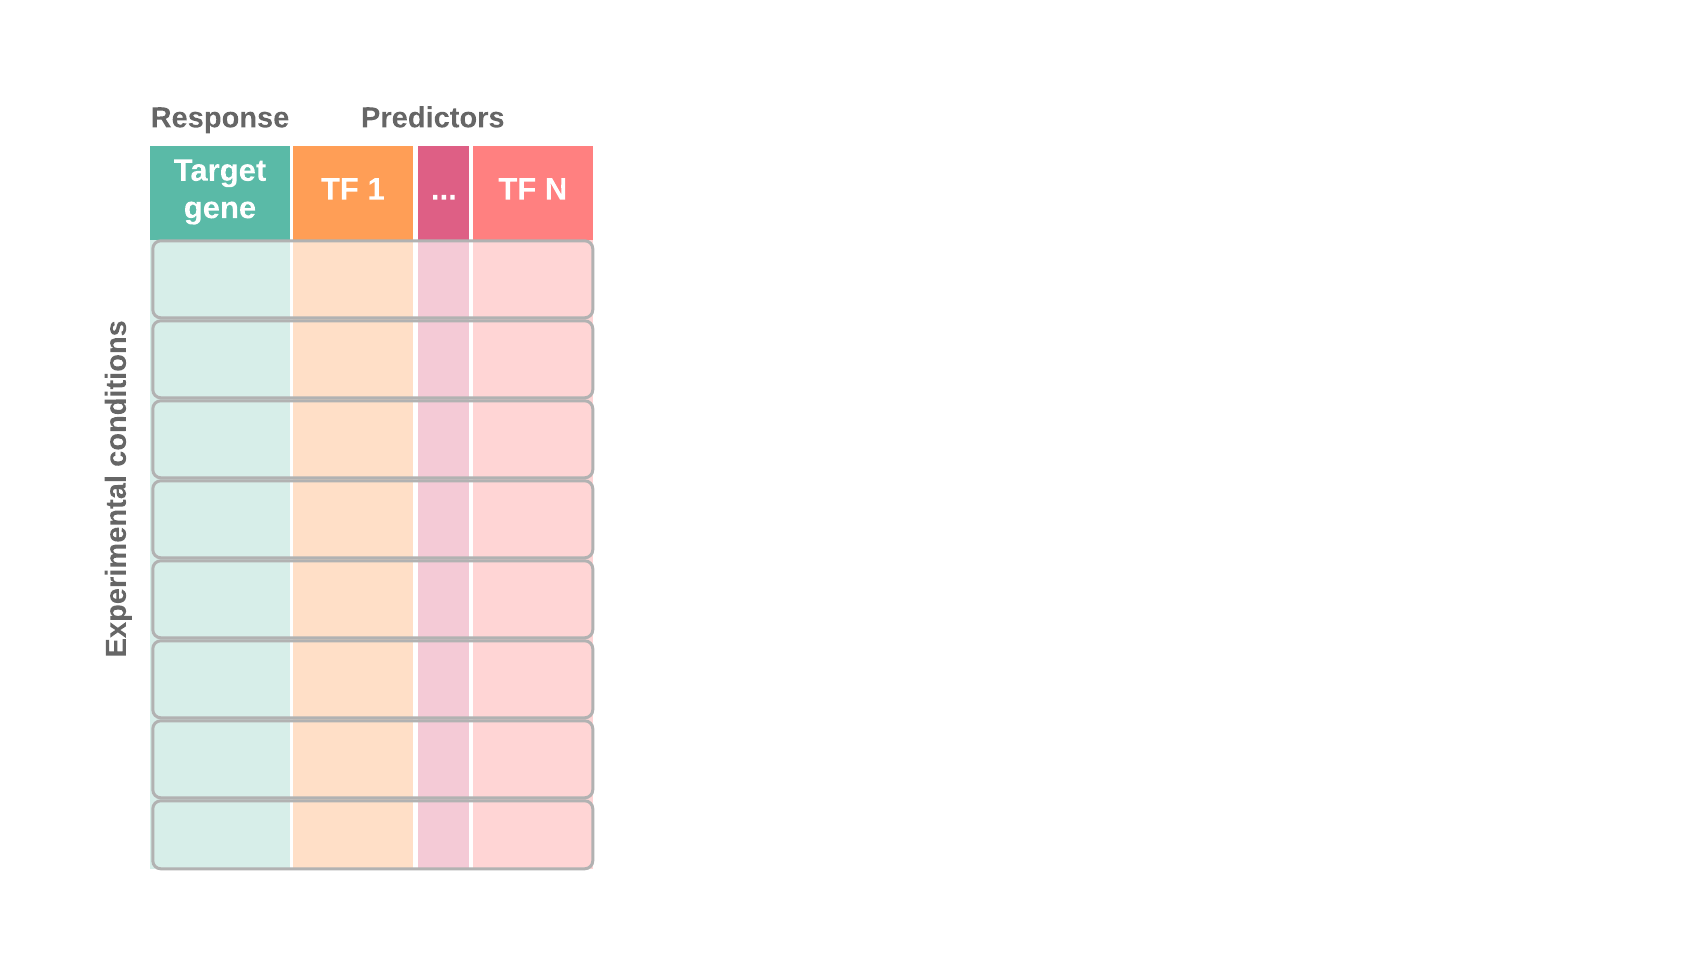
\includegraphics[scale = 0.38]{Figures/Regression/rf1.png}
        \onslide<2>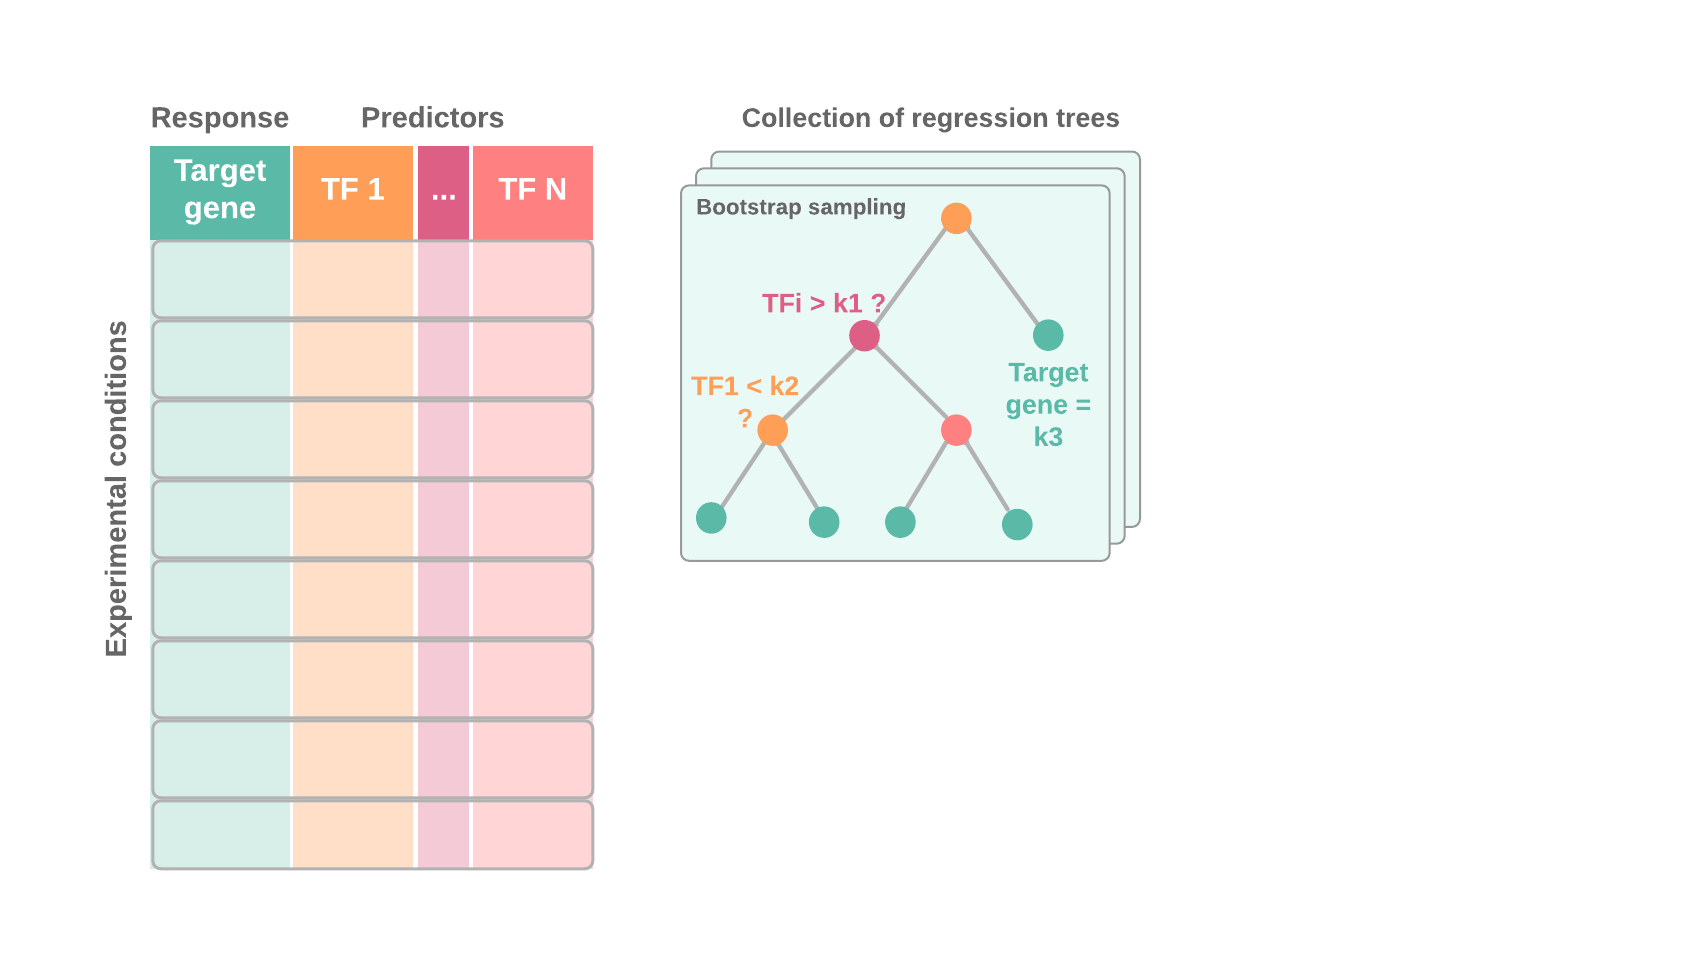
\includegraphics[scale = 0.38]{Figures/Regression/rf2.png}
        \onslide<3>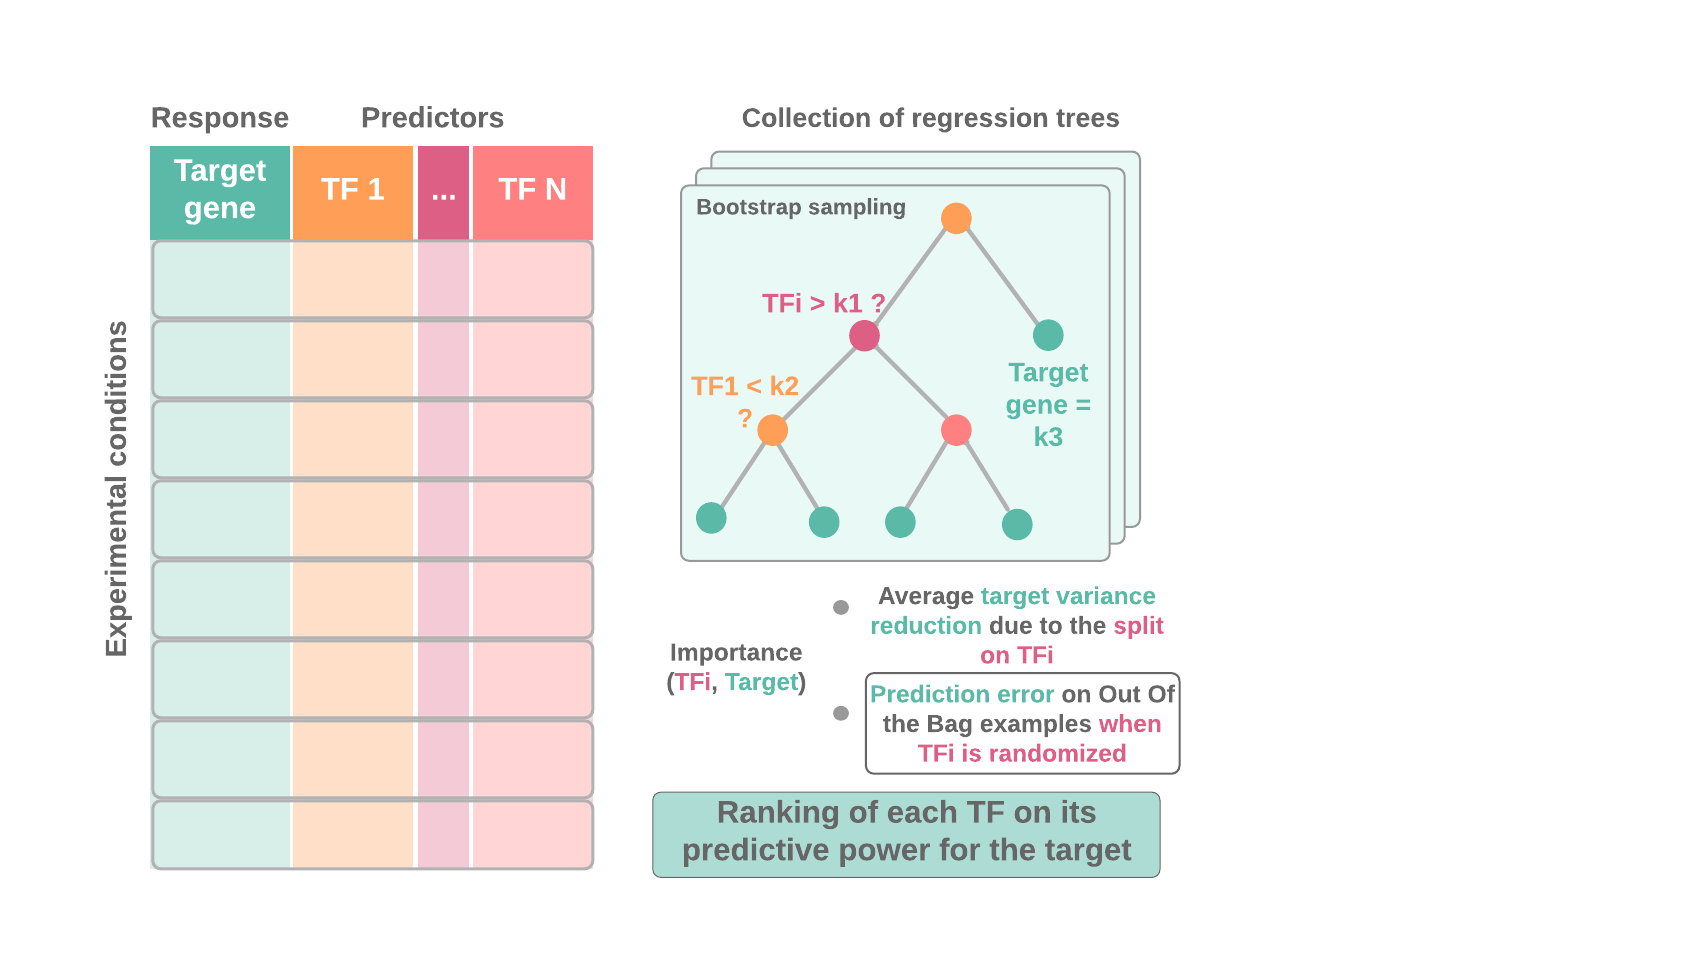
\includegraphics[scale = 0.38]{Figures/Regression/rf3.png}
        \onslide<4->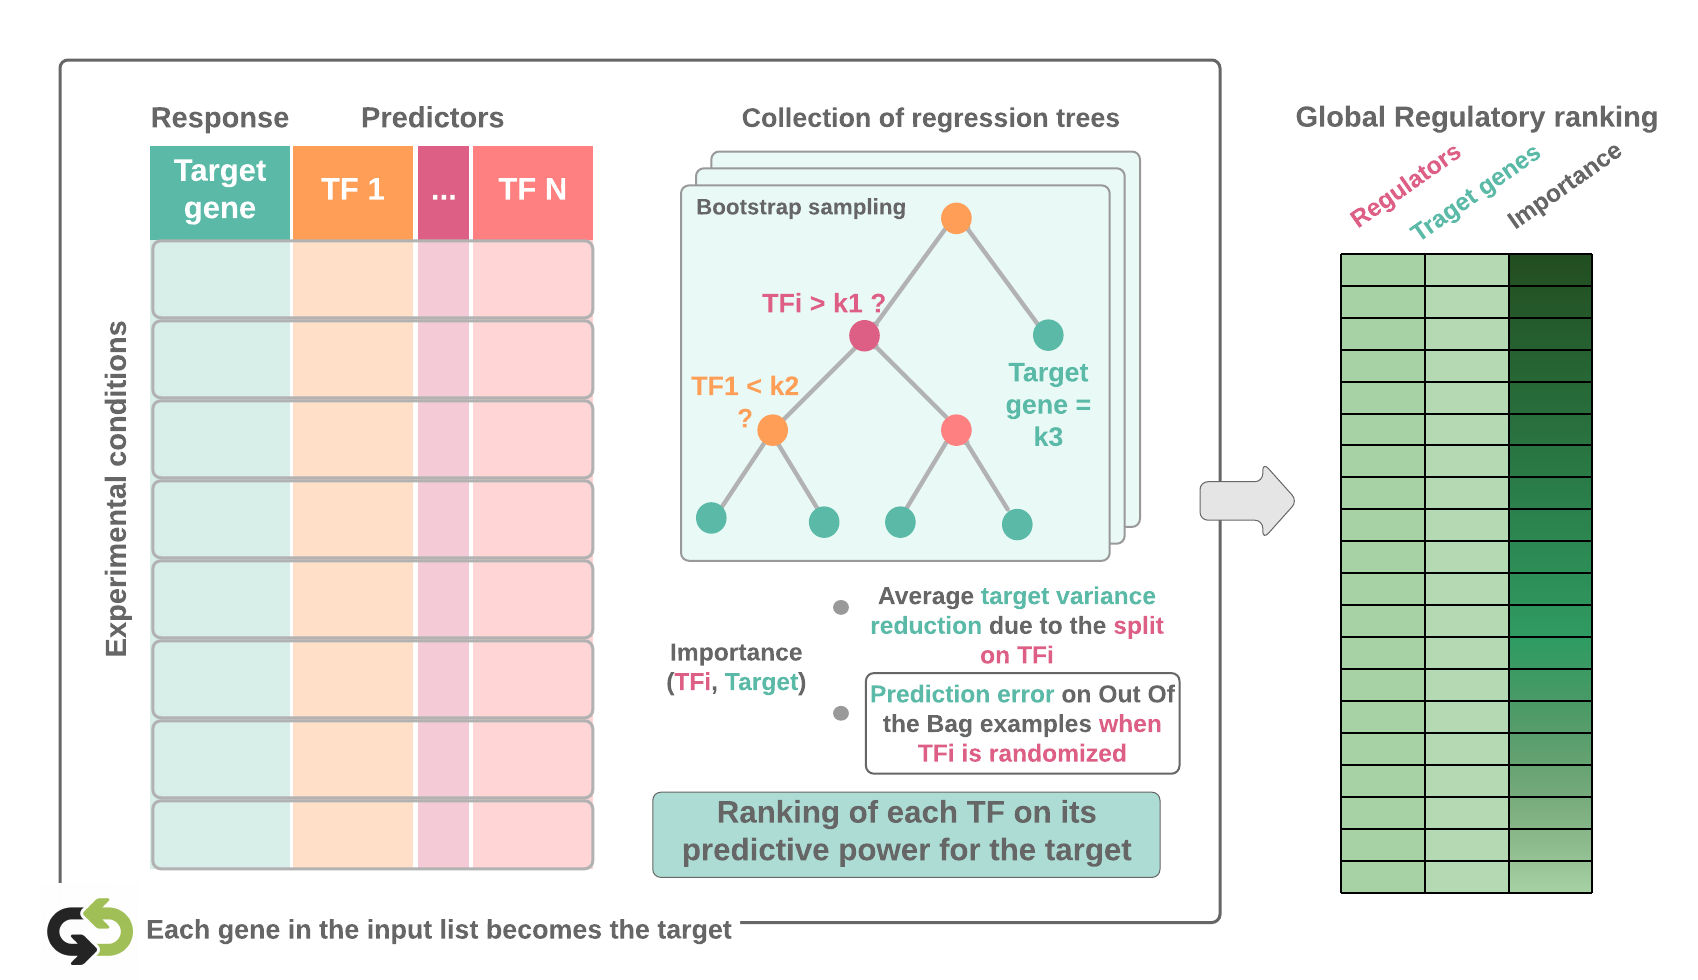
\includegraphics[scale = 0.38]{Figures/Regression/rf4.png}
    \end{overprint}
    \end{center}
\end{frame}





	
	\section{Validation et perspectives}
	
	%


\begin{frame}{Enrichir et valider un réseau inféré}


\small Les arêtes inférées peuvent être comparées à des \textbf{liens de régulation déjà documentés}, comme :


\begin{itemize} \small 
    \item Les interactions présentes dans la \textbf{litérature}
    \item Des \textbf{données de fixation} des TFs  \textit{in vivo} ou \textit{in vitro} CHIPSeq, DAPSeq
    \item L'\textbf{accessibilité de la chromatine} et footprinting : ATACSeq
    \item La \textbf{régulation \textit{in planta}} (induction de TF dans des protoplastes \cite{Bargmann2013}, expression de gènes cibles dans des lignées de mutants, etc) 
\end{itemize}
\vspace{-0.3cm}
\onslide<2->
\begin{block}{\small Quelques efforts de regroupement en bases de données:}
\begin{itemize}\small
    \item ConnecTF \cite{Brooks2020} (Arabidopsis, maïs)
    \item AtRegNet \cite{Palaniswamy2006} (Arabidopsis)
\end{itemize}
\end{block}
\end{frame}



\begin{frame}{Enrichir et valider un réseau inféré}

\begin{columns}
\begin{column}{.5\textwidth}
\vspace{-0.1cm}
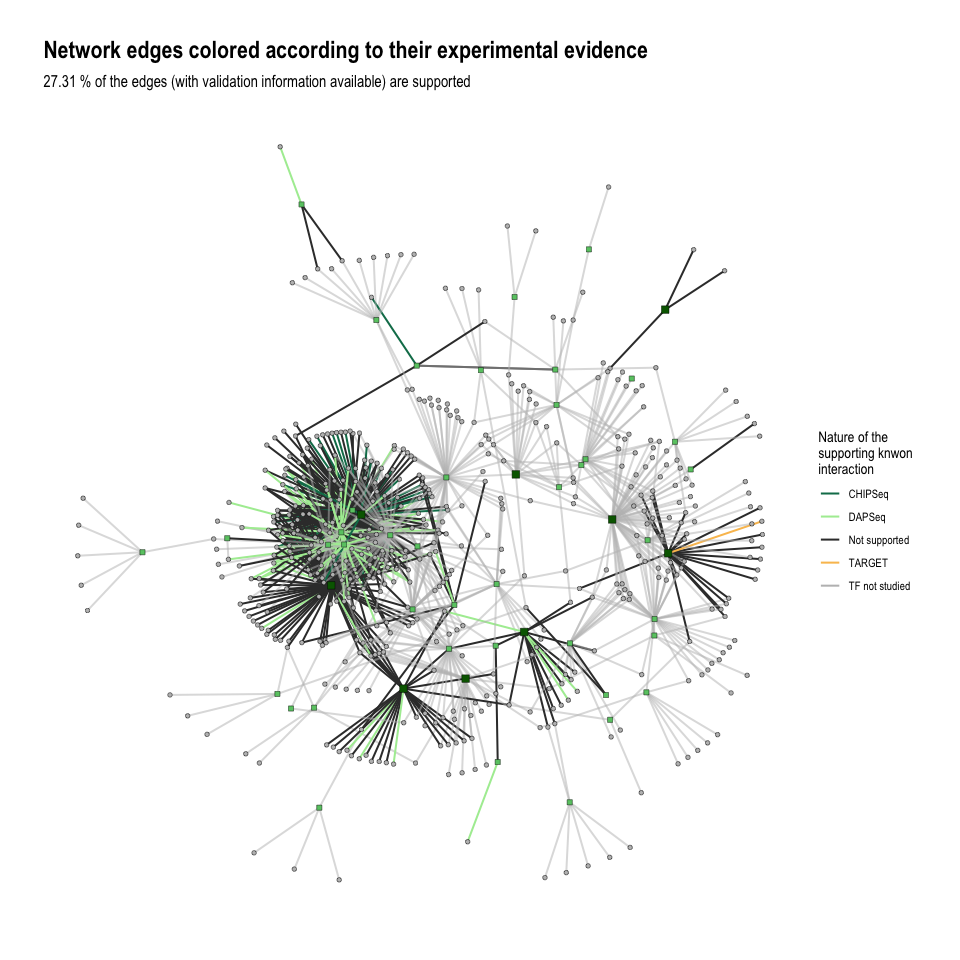
\includegraphics[scale = 0.21]{Figures/analyse/validation.png}
\end{column}
\begin{column}{.3\textwidth}
\vspace{-0.2cm}
\begin{block}{}
\scriptsize Ici, les arêtes d'un réseau prédit sont colorées suivant \textbf{leur confirmation par une expérience présente dans connecTF (DAPSeq, CHIPSeq, TARGET)}
\end{block}
\scriptsize Réseau inféré via GENIE3, validé via \href{https://oceanecsn.github.io/AraNetBench/}{AraNetBench}. \\ Arabidopsis sous stress osmotique, salin, et en température
\end{column}
\end{columns}
\end{frame}



\begin{frame}{Calculer des métriques de validation sur un réseau inféré}

\begin{columns}
\begin{column}{.48\textwidth}
\begin{itemize}\small
    \item \textbf{Vrais positifs - précision} : nombre d'arêtes prédites supportées par une information expérimentale (absolu, ou rapporté au nombre d'arêtes total qu'il est possible de valider)
    
    \item \textbf{Faux positifs, vrais négatifs, faux négatifs, rappel}
\end{itemize}
\onslide<3->
\begin{alertblock}{\small \danger Interprétation de ces métriques}\scriptsize
Ces données de validation sont \textbf{imparfaites}, elles contiennent des faux positifs, et faux négatifs : prudence
\end{alertblock}
\end{column}
\begin{column}{.48\textwidth}
\onslide<2->
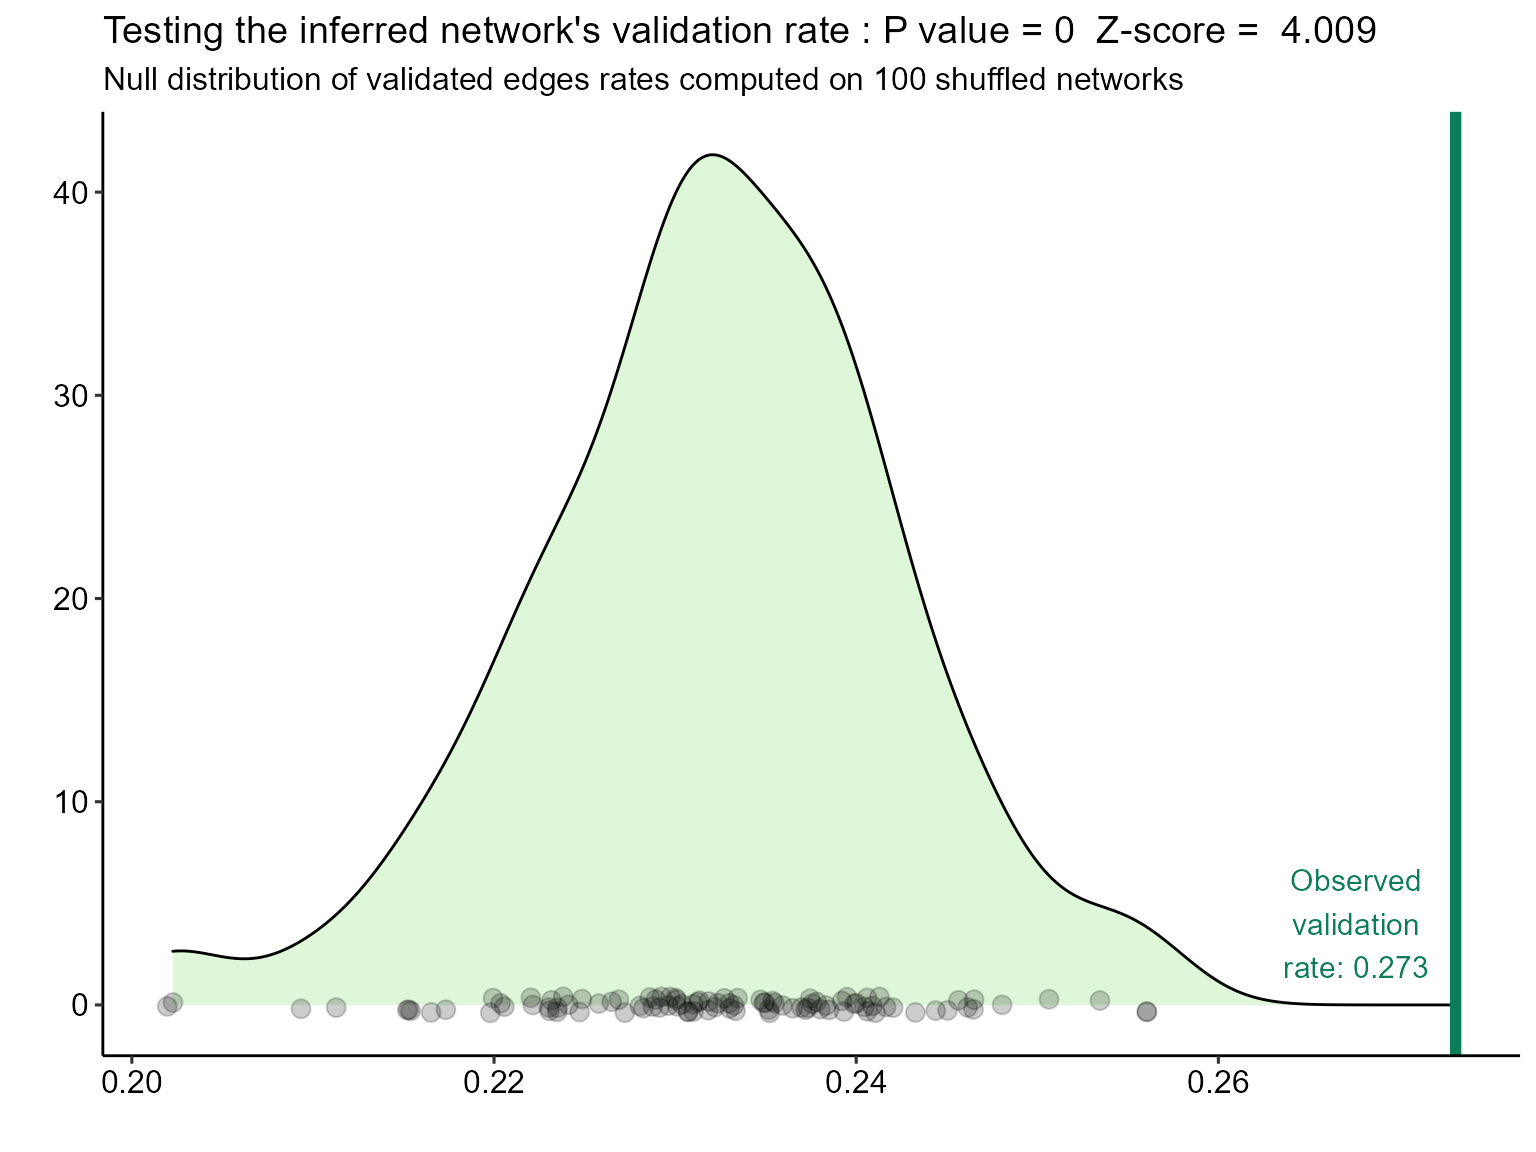
\includegraphics[scale = 0.3]{Figures/Regression/validationtest.png}
\end{column}
\end{columns}
\end{frame}

	
	%\section{Perspectives}


\begin{frame}{Principe de la régression pour les réseaux de régulation}
	
	\begin{center}
	\scriptsize 
	$regulators_{i}$ : niveaux d'expression des régulateurs transcriptionels dans la condition $i$
	
	$target_{i}$  : niveaux d'expression d'un gène cible dans la condition $i$
	\end{center}
	\vspace{-0.15cm}
	
	
	\begin{block}{}
	\begin{equation*}
	    target_{i} = \textcolor{orange}{\textbf{f}}(regulators_{i}) + \epsilon_i
	\end{equation*}
	\end{block}
	\vspace{0.25cm}

	\scriptsize 
	
	
	\textbf{La procédure de construction de réseau est la suivante} : 
	
	\begin{enumerate}
	    \item Pour chaque gène du jeu de données, ajuster à partir des valeurs d'expression la fonction \textcolor{orange}{\textbf{f}}
	    \item Extraire de \textcolor{orange}{\textbf{f}} les scores (ou valeur d'influence, importance, pouvoir prédictif) des régulateurs sur chaque gène du jeu de données 
	    \item Sélectionner les scores régulateurs-gènes cibles les plus forts pour construire le réseau final
	\end{enumerate}
\end{frame}



\begin{frame}{DIANE \scriptsize \cite{Cassan2021} }

\scriptsize \textbf{Dashboard for the Inference and Analysis of Networks from Expression data} 
\includegraphics[scale= 0.10]{Figures/Regression/hex-DIANE.png}

\scriptsize L'outil que vous utiliserez lors des TP-TD pour aller de données d'expression brutes jusqu'à l'inférence et l'analyses de réseau avec GENIE3.

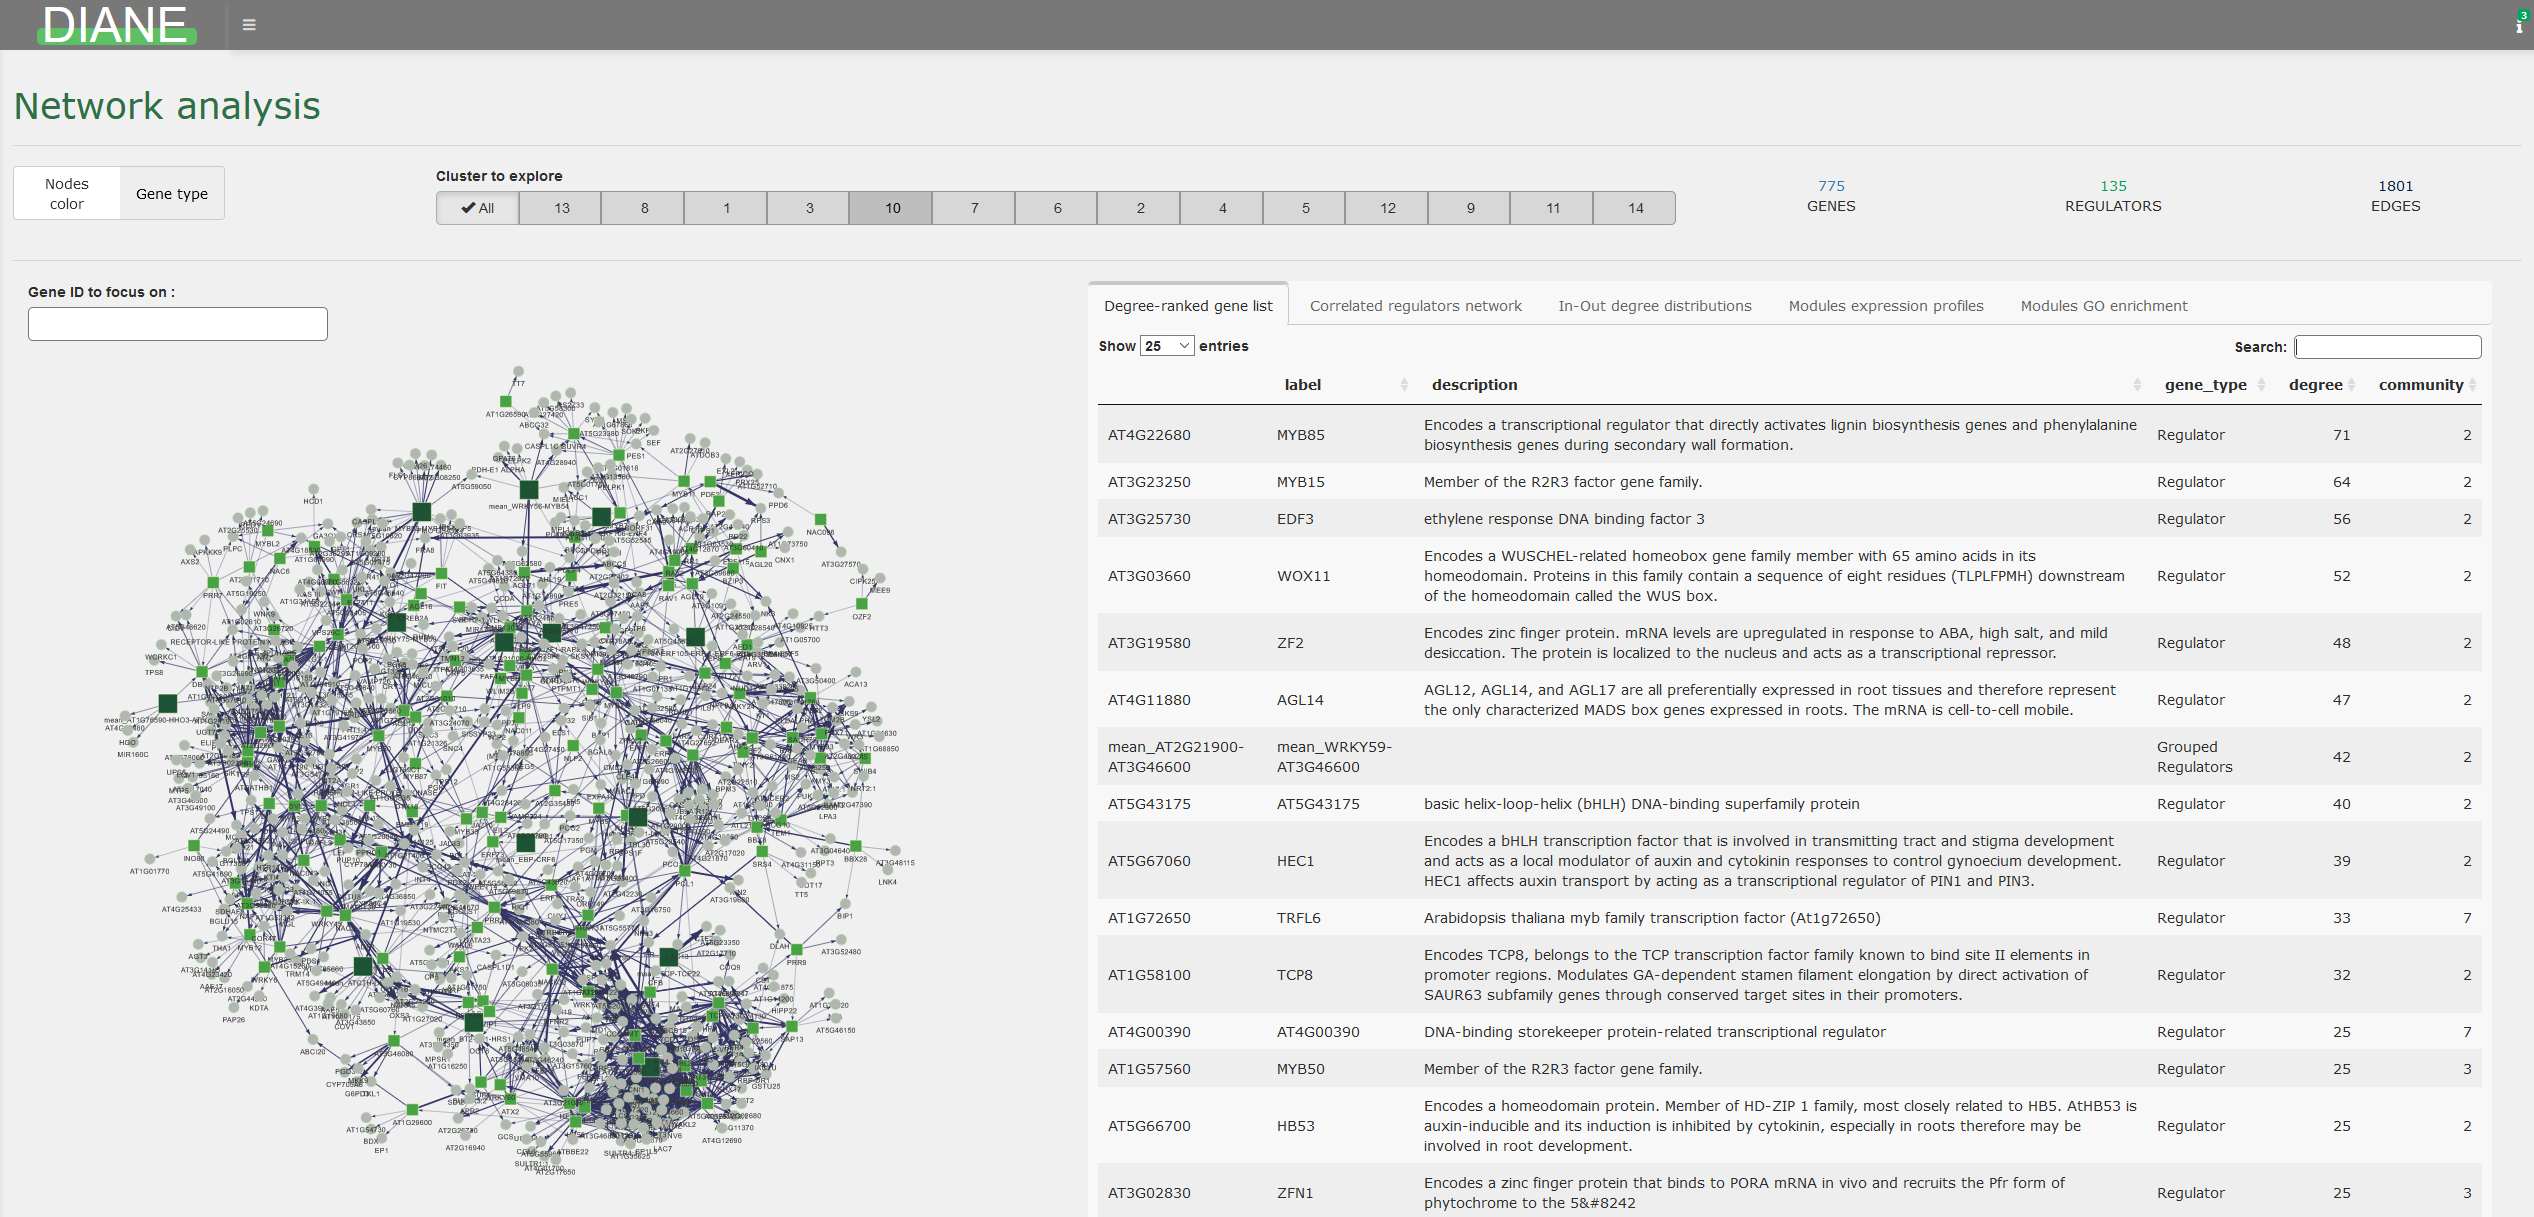
\includegraphics[scale = 0.2]{Figures/Regression/view_net.PNG}

\end{frame}






\begin{frame}{Enrichir et valider un réseau inféré}


\small Les arêtes inférées peuvent être comparées à des \textbf{liens de régulation déjà documentés}, comme :


\begin{itemize} \small 
    \item Les interactions présentes dans la \textbf{litérature}
    \item Des \textbf{données de fixation} des TFs  \textit{in vivo} ou \textit{in vitro} CHIPSeq, DAPSeq
    \item L'\textbf{accessibilité de la chromatine} et footprinting : ATACSeq
    \item La \textbf{régulation \textit{in planta}} (induction de TF dans des protoplastes \cite{Bargmann2013}, expression de gènes cibles dans des lignées de mutants, etc) 
\end{itemize}
\vspace{-0.3cm}
\onslide<2->
\begin{block}{\small Quelques efforts de regroupement en bases de données:}
\begin{itemize}\small
    \item ConnecTF \cite{Brooks2020} (Arabidopsis, maïs)
    \item AtRegNet \cite{Palaniswamy2006} (Arabidopsis)
\end{itemize}
\end{block}
\end{frame}



\begin{frame}{Enrichir et valider un réseau inféré}

\begin{columns}
\begin{column}{.5\textwidth}
\vspace{-0.1cm}
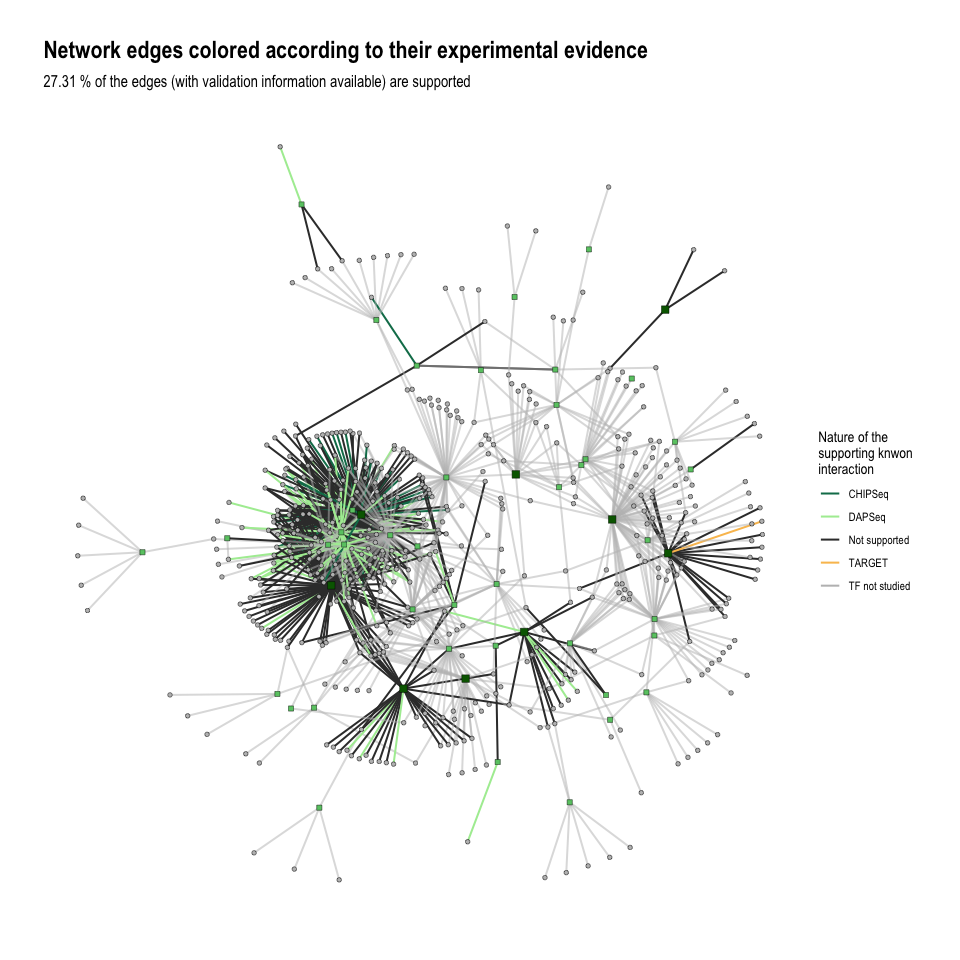
\includegraphics[scale = 0.21]{Figures/analyse/validation.png}
\end{column}
\begin{column}{.3\textwidth}
\vspace{-0.2cm}
\begin{block}{}
\scriptsize Ici, les arêtes d'un réseau prédit sont colorées suivant \textbf{leur confirmation par une expérience présente dans connecTF (DAPSeq, CHIPSeq, TARGET)}
\end{block}
\scriptsize Réseau inféré via GENIE3, validé via \href{https://oceanecsn.github.io/AraNetBench/}{AraNetBench}. \\ Arabidopsis sous stress osmotique, salin, et en température
\end{column}
\end{columns}
\end{frame}



\begin{frame}{Calculer des métriques de validation sur un réseau inféré}

\begin{columns}
\begin{column}{.48\textwidth}
\begin{itemize}\small
    \item \textbf{Vrais positifs - précision} : nombre d'arêtes prédites supportées par une information expérimentale (absolu, ou rapporté au nombre d'arêtes total qu'il est possible de valider)
    
    \item \textbf{Faux positifs, vrais négatifs, faux négatifs, rappel}
\end{itemize}
\onslide<3->
\begin{alertblock}{\small \danger Interprétation de ces métriques}\scriptsize
Ces données de validation sont \textbf{imparfaites}, elles contiennent des faux positifs, et faux négatifs : prudence
\end{alertblock}
\end{column}
\begin{column}{.48\textwidth}
\onslide<2->
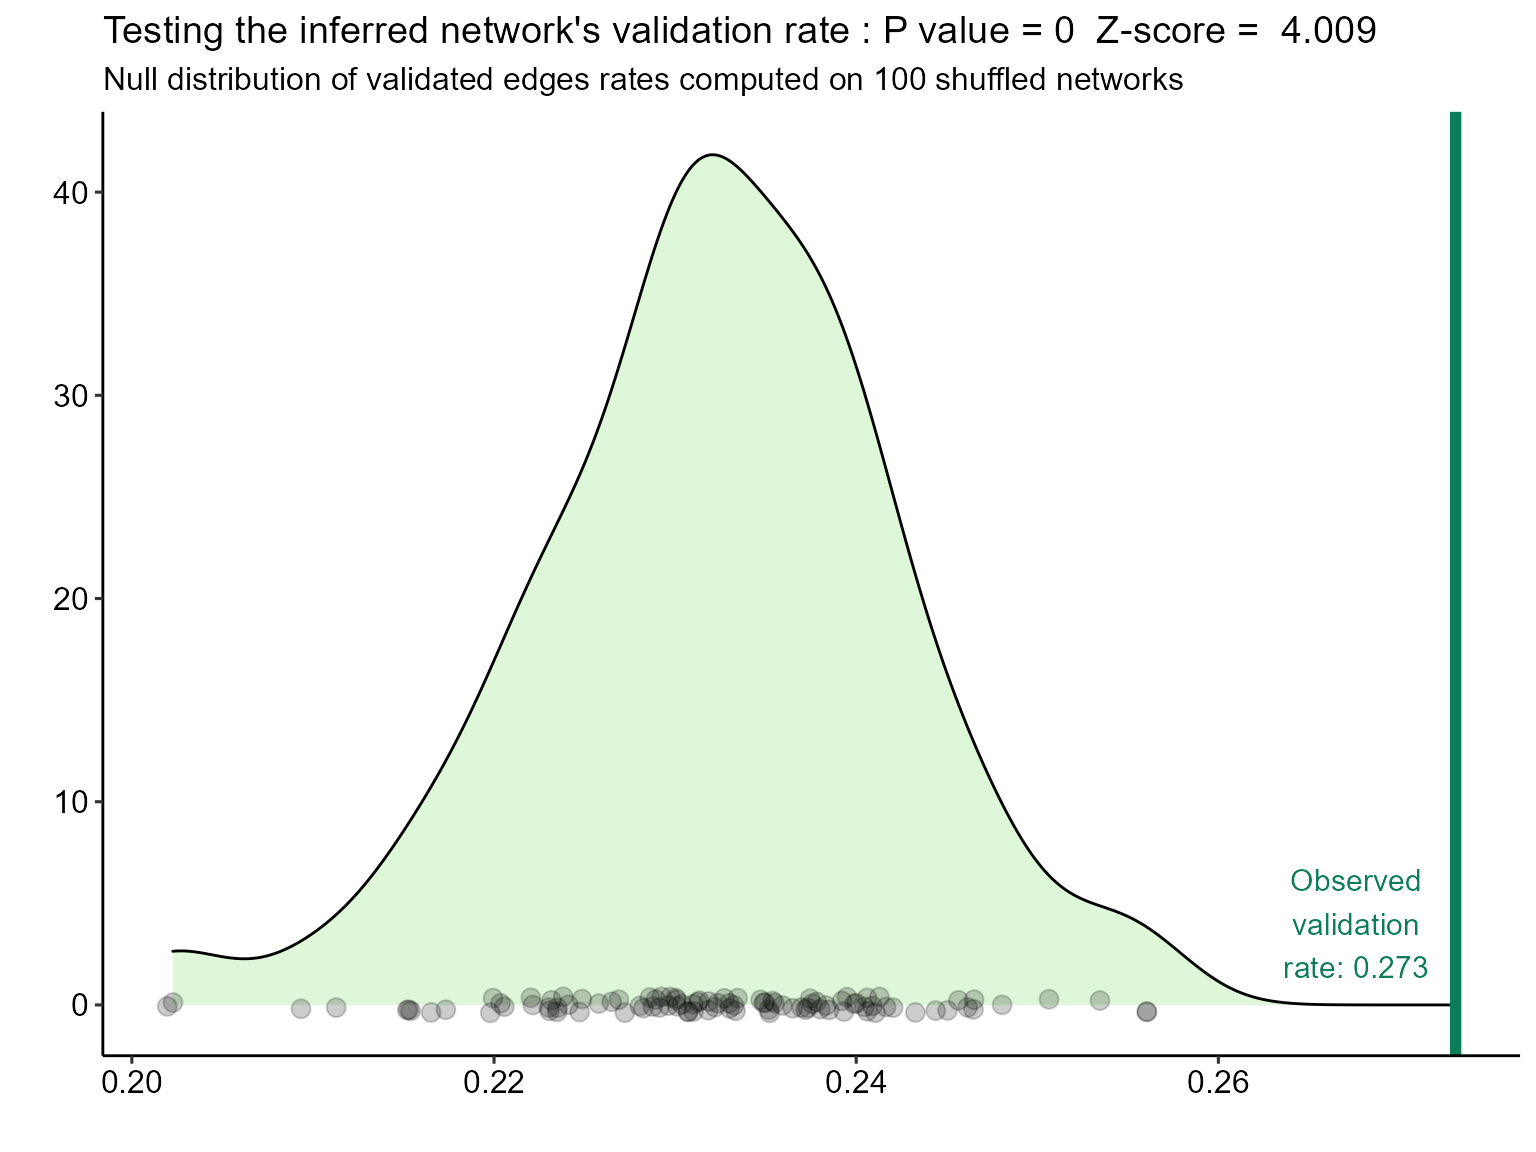
\includegraphics[scale = 0.3]{Figures/Regression/validationtest.png}
\end{column}
\end{columns}
\end{frame}



%\subsection{Analyse et validation de réseaux}



\begin{frame}{Analyser la topologie d'un réseau : détection de modules}

\begin{itemize}
    \item \small \textbf{Communautés} de gènes densément connectés, contenant des éventuels enrichissements ontologiques. \tiny{Conrad et al, BMC Syst. Biology 2018}
    \center
     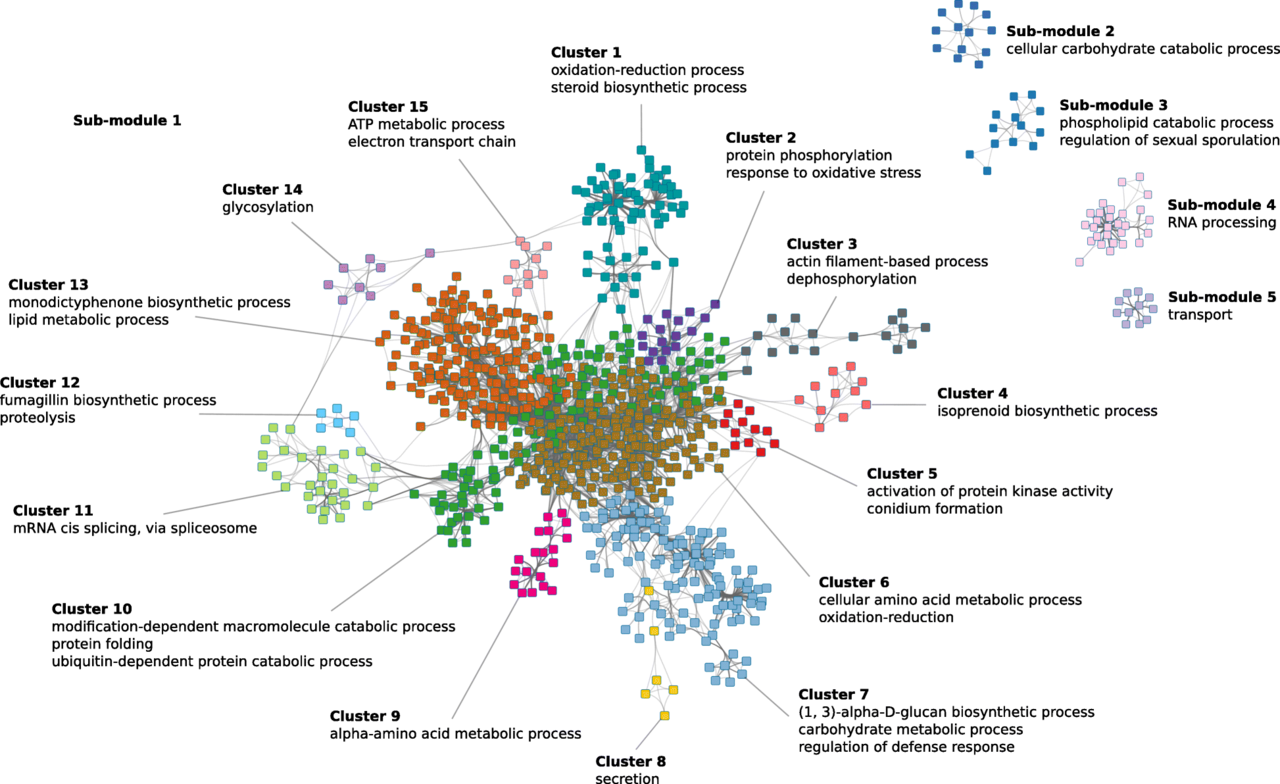
\includegraphics[scale = 0.195]{Figures/analyse/modules.png} 
     
    
\end{itemize}
	
\end{frame}


\begin{frame}{Analyser la topologie d'un réseau inféré : connectivité}

\begin{itemize}
 \item \small \textbf{Degré - centralité} : Les gènes montrant une connectivité remarquable dans le réseau sont de potentiels régulateurs clés
 
 \center
     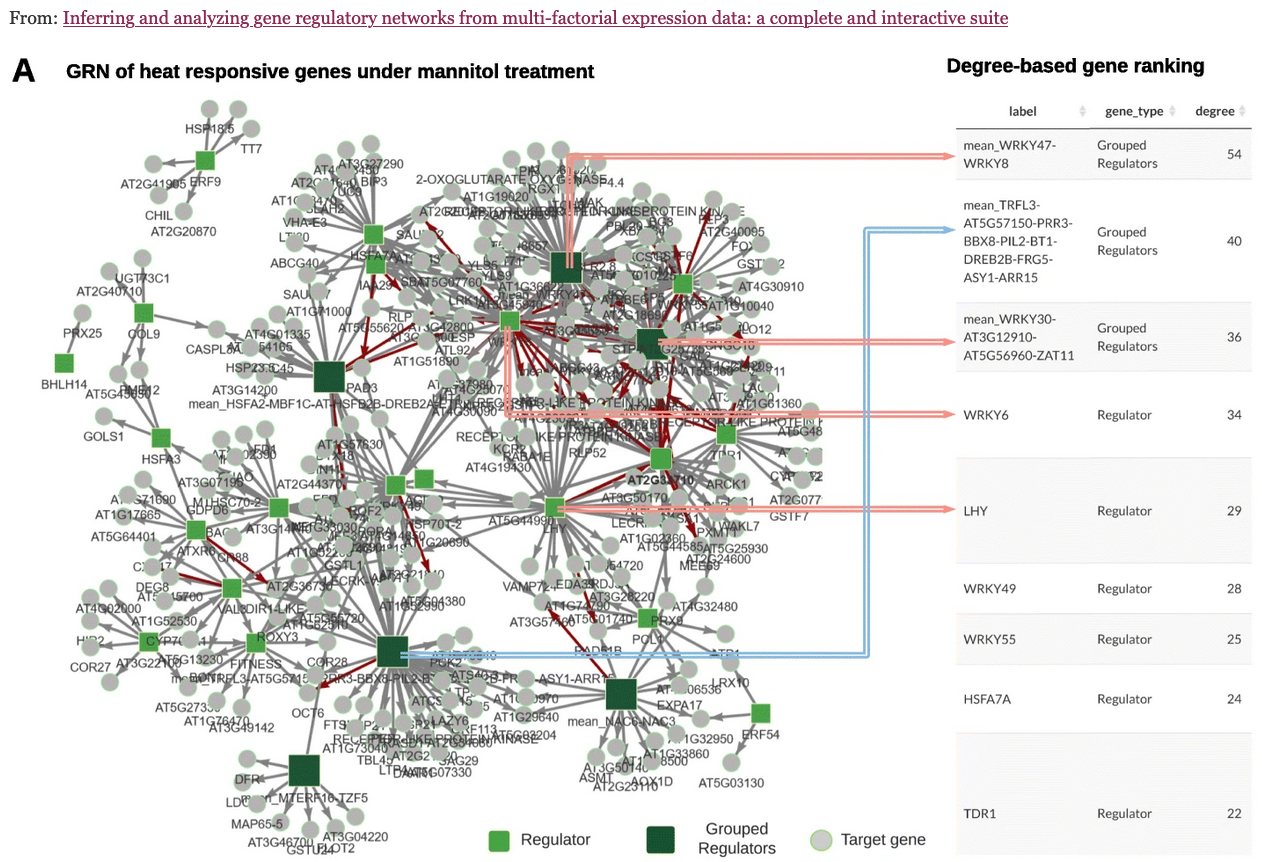
\includegraphics[scale = 0.17]{Figures/analyse/rankingTF.png}
    
\end{itemize}

\end{frame}


% conclusion / synthèse


\begin{frame}{Inférer des réseaux de régulation : un tâche encore complexe}
	
	\begin{enumerate}
	    \item Problème en grande dimension
	    
	    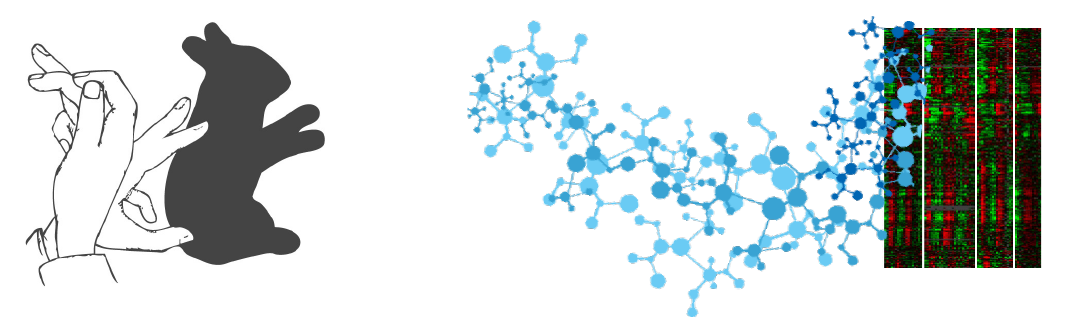
\includegraphics[scale=0.2]{Figures/Intro/shadowplay.png}
	    
	    
	    \item Manque de données de validation complètes et sûres pour étalonner les méthodes
	\end{enumerate}

\end{frame}




\begin{frame}{Combiner plusieurs approches d'inférence}

\scriptsize En 2012, les challenges \textbf{DREAM} ont évalué et combiné l'état de l'art des méthodes d'inférence  et conclu à un apport significatif de la combinaison de plusieurs méthodes [Marbach et al., 2012]

\centering
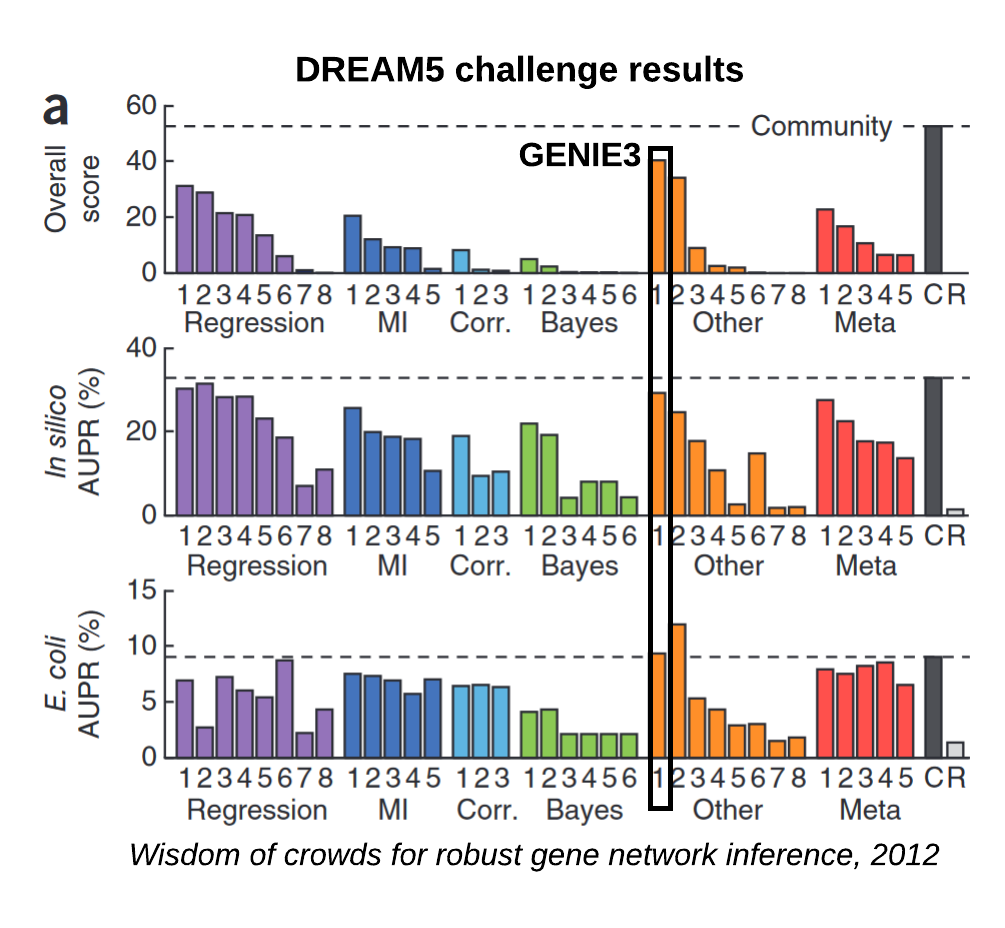
\includegraphics[scale = 0.38]{Figures/Regression/dream5.png}
\end{frame}



\begin{frame}{Utilité de ces analyses pour la biologie des systèmes}

\textbf{L'analyse des réseaux inférés peut permettre de:}
    \begin{itemize} \small
    \item Conforter et approfondir des connaissances existantes en biologie des systèmes
        \item Découvrir de nouveaux gènes candidats contrôlant des réponses d'intérêt, après validation expérimentale et étude fonctionnelle
    \end{itemize}
    
    \vspace{0.5cm}
    \begin{alertblock}{Accomplissements de l'inférence de réseaux}
	Meilleure compréhension des systèmes vivants, solutions pour améliorer la résilience d'un organisme à une contrainte environnementale ou à des pathologies
	\end{alertblock}
	
    
\end{frame}
	




\begin{frame}[allowframebreaks]
    \frametitle{References}
    \setbeamertemplate{bibliography item}[triangle]
    \scriptsize
    \bibliographystyle{apalike}
    \bibliography{biblio}
\end{frame}


\end{document}